\documentclass[final]{beamer} 
\usetheme[headheight=10cm,footheight=5cm]{boxes}
\usetheme{toby}
%\usepackage{times}
\usepackage{etex}
\usepackage{amsmath,amssymb}
\usepackage[latin1]{inputenc}
\usepackage[english]{babel}
\usepackage{helvet}
\usepackage[T1]{fontenc}
\usepackage{textcomp}
\usepackage[orientation=landscape,size=a0,scale=1.4,debug]{beamerposter}   % e.g. for DIN-A0 poster
\usepackage{exscale}
\usepackage{pst-plot}
\usepackage{pstricks-add}
\usepackage{epsfig}
\usepackage{eulervm}
\usepackage{tikz}
\usepackage{array}
\usepackage{subfigure}
\usepackage{graphicx}
  
% \usepackage[size=custom,width=3.0,height=120,scale=2,debug]{beamerposter}  % e.g. custom size poster

\usepackage{beamerthemetoby}

\def\x{{\mathbf x}}
\def\z{{\mathbf z}}
\def\l{{\ell}}
\def\1{{\mathbf 1}}
\def\0{{\mathbf 0}}
\def\a{{\mathbf a}}
%\def\c{{\mathbf c}}
\def\p{{\mathbf p}}
\def\v{{\mathbf v}}
\def\n{{\mathbf n}}
\def\X{{\mathbf X}}
\def\Z{{\mathbf Z}}
\def\eg{e.g.}
\def\ZZ{{\mathcal Z}}
\def\hatx{{\mathbf {\hat x}}}
\def\hatf{{ \hat f}}
\def\hatw{{\bf \hat w}}
\def\hati{{\hat{\imath}}}
\def\tildej{\tilde{\jmath}}
\def\tildel{\tilde{\ell}}
\def\hatX{{\bf \hat X}}
\def\hatb{{\hat b}}
\def\ae{\text{~~a.e.}}
\def\as{\text{~~a.s.}}
\def\hatalpha{\mbox{\boldmath${\hat \alpha}$}}
\def\tildealpha{\mbox{\boldmath${\tilde \alpha}$}}
\def\tildebeta{\mbox{\boldmath${\tilde \beta}$}}
\def\hatDelta{\mbox{\boldmath${\hat \Delta}$}}
\def\Lambdab{{\boldsymbol\Lambda}}
\def\lambdab{{\boldsymbol\lambda}}
\def\kappab{{\boldsymbol\kappa}}
\def\rhob{{\boldsymbol\rho}}
\def\taub{{\boldsymbol\tau}}

\def\xib{{\boldsymbol\xi}}
\def\xibbar{\tilde{\boldsymbol{\xi}}}
\def\nub{{\boldsymbol\nu}}
\def\Gammab{{\boldsymbol\Gamma}}
\def\Thetab{{\boldsymbol\Theta}}
\def\Sigmab{{\boldsymbol\Sigma}}
\def\Deltab{{\boldsymbol\Delta}}
\def\betab{{\boldsymbol\beta}}
\def\epsilonb{{\boldsymbol\varepsilon}}
\def\varepsilonb{{\boldsymbol\varepsilon}}
\def\alphab{{\boldsymbol\alpha}}
\def\thetab{{\boldsymbol\theta}}
\def\gammab{{\boldsymbol\gamma}}
\def\alphabtilde{{\boldsymbol\tilde{\alpha}}}
\def\hatlambdab{{\boldsymbol{\hat\lambda}}}
\def\Gammab{{\boldsymbol\Gamma}}
\def\tildeGammab{{\bf \tilde{\boldsymbol\Gamma}}}
\def\y{{\mathbf y}}
\def\FFF{\text{F}}
\def\w{{\mathbf w}}
\def\vw{{\mathbf w}}
\def\D{{\mathbf D}}
\def\mX{{\mathbf D}}
\def\Y{{\mathbf Y}}
\def\YY{{\mathcal Y}}
\def\M{{\mathbf M}}
\def\B{{\mathbf B}}
\def\Q{{\mathbf Q}}
\def\C{{\mathbf C}}
\def\W{{\mathbf W}}
\def\d{{\mathbf d}}
\def\E{{\mathbb E}}
\def\PPP{{\mathbb E}}
\def\EE{{\mathbf E}}
\def\O{{O}}
\def\N{{\mathcal N}}
\def\o{{\mathcal o}}
\def\s{{\mathbf s}}
\def\CC{{\mathcal C}}
\def\VV{{\mathcal V}}
\def\NN{{\mathcal N}}
\def\KK{{\mathcal K}}
\def\CCC{{C}}
\def\L{{\mathcal L}}
\def\P{{\mathcal P}}
\def\PP{{\mathbf P}}
\def\PPP{{\mathbb P}}
\def\R{{\mathbf R}}
\def\RR{{\mathcal R}}
\def\S{{\mathcal S}}
\def\SS{{\mathbf SS}}
\def\H{{\mathcal H}}
\def\d{{\mathbf d}}
\def\e{{\mathbf e}}
\def\b{{\mathbf b}}
\def\cc{{\mathbf c}}
\def\u{{\mathbf u}}
\def\m{{\mathbf m}}
\def\hatD{{\bf \hat D}}
\def\tildeD{{\mathbf{\tilde{D}}}}
\def\tildeB{{\mathbf{\tilde{B}}}}
\def\tildeC{{\mathbf{\tilde{C}}}}
\def\tildex{{\mathbf{\tilde{x}}}}
\def\tildef{{ \tilde f}}
\def\hatE{{\bf \hat E}}
\def\hate{{\bf \hat e}}
\def\hatd{{\bf \hat d}}
\def\hatf{{ \hat f}}
\def\tilded{{\bf \tilde d}}
\def\Real{{\mathbb R}}
\def\r{{\mathbf r}}
\def\U{{\mathbf U}}
\def\UY{{\mathcal U}}
\def\u{{\mathbf u}}
\def\A{{\mathbf A}}
\def\G{{\mathbb G}}
\def\GG{{\mathcal G}}
\def\AA{{\mathcal A}}
\def\FF{{\mathcal F}}
\def\DD{{\mathcal D}}
\def\XX{{\mathcal X}}
\def\WW{{\mathcal W}}
\def\V{{\mathbf V}}
\def\K{{\mathbf K}}
\def\KK{{\mathcal K}}
\def\T{{\mathbf T}}
\def\TT{{\mathcal T}}
\def\I{{\mathbf I}}
\def\one{{\mathbb 1}}
\def\argmin{\operatornamewithlimits{arg\,min}}
\def\liminf{\operatornamewithlimits{lim\,inf}}
\def\argmax{\operatornamewithlimits{arg\,max}}
\def\Var{\operatorname{Var}}
\def\diag{\operatorname{diag}}
\def\trace{\operatorname{Tr}}
\def\range{\operatorname{range}}
\def\vec{\operatorname{vec}}
\def\sign{\operatorname{sign}}
\def\FL{\operatorname{FL}}
\def\corr{\operatorname{corr}}
\def\cov{\operatorname{cov}}
\def\st{~~\text{s.t.}~~}
\def\defin{\triangleq}
%\def\TODO{ {\color{red} TODO }}
\newcommand{\TODO}[1]{{\textbf{\color{red} TODO: #1}}}

\def\gi{ {\scriptscriptstyle \hspace*{-0.002cm}\mid\hspace*{-0.008cm}}  g}
\def\hi{  {\scriptscriptstyle \hspace*{-0.002cm}\mid\hspace*{-0.008cm}}  h}

%\renewcommand{\cite}{\citep}
\newcommand{\refEq}{\ref}
%\renewenvironment{displaymath}{\begin{equation}}{\end{equation}}
%\renewenvironment{multline*}{\begin{multline}}{\end{multline}}

%\renewcommand{\cite}{\citep}
% \newcommand{\citet}{\emcite}
% \renewenvironment{displaymath}{\begin{equation}}{\end{equation}}
%:w\renewenvironment{multline*}{\begin{multline}}{\end{multline}}

% \newtheorem{example}{Example} 
% 

%\newcommand{\InSet}[1]{\text{\textlbrackdbl} 1;#1 \text{\textrbrackdbl}}
\newcommand{\InSet}[1]{\llbracket 1;#1 \rrbracket}
\newcommand{\IntSet}[1]{\llbracket 1;#1 \rrbracket}
\renewcommand{\bf}{\textbf}

\newcommand{\Norm}[1]{\|#1\|}
\newcommand{\DualNorm}[1]{\|#1\|_{\ast}}
\newcommand{\NormUn}[1]{\|#1\|_1}
\newcommand{\NormDeux}[1]{\|#1\|_2}
\newcommand{\NormInf}[1]{\|#1\|_{\infty}}
\newcommand{\NormFro}[1]{\|#1\|_{\text{F}}}
\newcommand{\NormFrob}[1]{\|#1\|_{\text{F}}}

\newcommand{\INPUT}{ {\bfseries Input: }}

\newcommand{\rred}[1]{{\textcolor{red}{#1}}}
\definecolorset{rgb}{}{}{inriablue,0.35,0.31,0.75}
\newcommand{\bblue}[1]{{\textcolor{inriablue}{#1}}}

\title[]{\veryHuge{Clusterpath: an Algorithm for Clustering using Convex Fusion Penalties}}
\author[]{Toby Dylan Hocking \and
      Armand Joulin \and
      Francis Bach \and
      Jean-Philippe Vert}
    \institute[Sierra]{~}%DONT DELETE THIS
\begin{document}
\begin{frame}{} 
\begin{columns}[T]
\hfill
\begin{column}{0.315\paperwidth}
% \begin{block}{One minute overview}
% \begin{itemize}
% \item Solving large-scale \rred{structured sparse} regularized problems.
% \item Use of (accelerated) \rred{proximal gradient methods}.
% \item Proximal operator solved with \rred{network flow optimization}.
% \end{itemize}
% \end{block}
\begin{block}{The clustering problem: existing methods}
  \begin{itemize}
  \item Clustering: assign labels to $n$ points in $p$ dimensions
    $X\in\RR^{n\times p}$.
  \item Methods:
    \begin{itemize}
  \item K-means
  \item Hierarchical
  \item Mixture models
  \item Spectral (Ng \emph{et al.} 2001)
  \item ... 
    \end{itemize}
    \item Issues:
    \begin{itemize}
    \item Hierarchy
    \item Convexity
    \item Greediness
    \item Stability
  \end{itemize}
  \end{itemize}
\end{block}


\begin{block}{Clusterpath: a convex relaxation of hierarchical
    clustering}
\begin{itemize}
\item A hard-thresholding of differences is a combinatorial problem:
$
 \min_{    \alpha\in\RR^{n\times p}}       ||\alpha-X||_F^2 \text{  subject to  }
\sum_{i<j}1_{\alpha_i\neq\alpha_j} \leq t$
\item Relaxation:$\sum_{i<j}||\alpha_i-\alpha_j||_q w_{ij}\leq t$
\item The Lagrange form is useful for optimization algorithms:
$$
\alpha^*(\lambda,q,w)=\operatorname{argmin}_{\alpha\in\RR^{n\times p}}
\frac 1 2||\alpha-X||_F^2+\lambda\sum_{i<j}||\alpha_i-\alpha_j||_q w_{ij}
$$
\item The \alert<1>{clusterpath} the continuous path of optimal
  $\alpha^*$ obtained by varying $\lambda$, for fixed weights
  $w_{ij}\in\RR^+$ and norm $q\in\{1,2,\infty\}$.
\item
 Related work: ``fused lasso'' Tibshirani and Saunders (2005),
``grouping pursuit'' Shen and Huang (2010), ``sum of norms'' Lindsten
\emph{et al.}  (2011).
\end{itemize}


\end{block}


\end{column}\hfill

\begin{column}{0.315\linewidth}
\begin{block}{Hierarchical norms: Jenatton et al, ICML 2010} 
\begin{itemize}
   \item A set of groups is \rred{tree-structured} if $$\forall g,h \in \GG,~~ g \cap h = \emptyset ~~\text{or}~~ g \subset h ~~\text{or}~~ h \subset g.$$
   \item Order the groups $g_1,\ldots,g_m$ \rred{from the leaves to the root}.
   \item The proximal operator admits a \rred{closed form}: $$\text{Prox}_{\lambda\Omega} = \text{Prox}^{g_1} \circ \ldots \circ \text{Prox}^{g_m}.$$
   \item Sequence of small proximal operators/projections.
   \item \rred{$O(p)$ operations} for $\ell_2$-norms ($O(pd)$ for $\ell_\infty$-norms).
\end{itemize}
\end{block}

\begin{block}{Outline of the $\ell_1$ path algorithm}
$$0 = \alpha_i - X_i + 
\lambda \sum_{j\neq i\atop \alpha_i \neq \alpha_j}w_{ij}
\operatorname{sign}({\alpha_i-\alpha_j}) + 
\lambda \sum_{j\neq i \atop \alpha_i = \alpha_j}w_{ij} \beta_{ij},$$
with $|\beta_{ij}|\leq 1$ and $\beta_{ij}=-\beta_{ji}$ (Hoefling 2009).
\begin{enumerate}
\item For $\lambda=0$ the solution $\alpha=X$ is optimal. We
  initialize the clusters $C_i = \{i\}$ and coefficients $\alpha_i =
  X_i$ for all $i$.
\item As $\lambda$ increases, the solutions will follow straight
  lines until they hit.
\item Taking the derivative of the optimality condition with respect
  to $\lambda$ leads to the following expression for the velocity of
  the initial clusters:
$$v_i = \sum_{j\neq i}w_{ij}\sign(\alpha_j-\alpha_i)$$
\item When 2 clusters $C_1$ and $C_2$ hit, they will merge to form a
  new cluster $C = C_1\cup C_2$ and take a new velocity:
$$v_C = \frac{
|C_1|v_1 + |C_2|v_2
}{
|C_1|+|C_2|
}$$
\item Stop when all the points merge at the mean $\overline X$.
\item Combine dimensions using $\lambda$ values.
\end{enumerate}

\end{block}

% Created by tikzDevice version 0.6.1 on 2011-06-26 17:49:00
% !TEX encoding = UTF-8 Unicode
\begin{tikzpicture}[x=1pt,y=1pt]
\definecolor[named]{drawColor}{rgb}{0.00,0.00,0.00}
\definecolor[named]{fillColor}{rgb}{1.00,1.00,1.00}
\fill[color=fillColor,] (0,0) rectangle (722.70,433.62);
\begin{scope}
\path[clip] (  0.00,  0.00) rectangle (722.70,433.62);
\end{scope}
\begin{scope}
\path[clip] (  0.00,  0.00) rectangle (722.70,433.62);
\end{scope}
\begin{scope}
\path[clip] (  0.00,  0.00) rectangle (722.70,433.62);
\end{scope}
\begin{scope}
\path[clip] (  0.00,  0.00) rectangle (722.70,433.62);
\end{scope}
\begin{scope}
\path[clip] (  0.00,  0.00) rectangle (722.70,433.62);
\end{scope}
\begin{scope}
\path[clip] (  0.00,  0.00) rectangle (722.70,433.62);
\end{scope}
\begin{scope}
\path[clip] (  0.00,  0.00) rectangle (722.70,433.62);
\end{scope}
\begin{scope}
\path[clip] (  0.00,  0.00) rectangle (722.70,433.62);
\end{scope}
\begin{scope}
\path[clip] (  0.00,  0.00) rectangle (722.70,433.62);
\definecolor[named]{fillColor}{rgb}{1.00,1.00,1.00}

\draw[fill=fillColor,draw opacity=0.00,] (  0.00,  0.00) rectangle (722.70,433.62);
\end{scope}
\begin{scope}
\path[clip] (  0.00,  0.00) rectangle (722.70,433.62);
\definecolor[named]{drawColor}{rgb}{0.00,0.00,0.00}

\node[color=drawColor,anchor=base,inner sep=0pt, outer sep=0pt, scale=  0.60] at (356.02,392.92) {$\ell_1$ clusterpath of 10 points in 2d%
};
\end{scope}
\begin{scope}
\path[clip] (  0.00,  0.00) rectangle (722.70,433.62);
\definecolor[named]{drawColor}{rgb}{0.00,0.00,0.00}

\node[color=drawColor,anchor=base,inner sep=0pt, outer sep=0pt, scale=  0.42] at (356.02,  7.23) {$\alpha^2$\hspace{2in}%
};
\end{scope}
\begin{scope}
\path[clip] (  0.00,  0.00) rectangle (722.70,433.62);
\definecolor[named]{drawColor}{rgb}{0.00,0.00,0.00}

\node[rotate= 90.00,color=drawColor,anchor=base,inner sep=0pt, outer sep=0pt, scale=  0.50] at ( 25.48,208.89) {$\alpha^1$%
};
\end{scope}
\begin{scope}
\path[clip] (  0.00,  0.00) rectangle (722.70,433.62);
\end{scope}
\begin{scope}
\path[clip] ( 44.91,385.70) rectangle ( 72.08,385.70);
\end{scope}
\begin{scope}
\path[clip] (  0.00,  0.00) rectangle (722.70,433.62);
\end{scope}
\begin{scope}
\path[clip] ( 44.91,385.70) rectangle ( 72.08,385.70);
\end{scope}
\begin{scope}
\path[clip] (  0.00,  0.00) rectangle (722.70,433.62);
\end{scope}
\begin{scope}
\path[clip] (  0.00,  0.00) rectangle (722.70,433.62);
\end{scope}
\begin{scope}
\path[clip] (  0.00,  0.00) rectangle (722.70,433.62);
\end{scope}
\begin{scope}
\path[clip] ( 44.91, 55.41) rectangle ( 72.08, 55.41);
\end{scope}
\begin{scope}
\path[clip] (  0.00,  0.00) rectangle (722.70,433.62);
\end{scope}
\begin{scope}
\path[clip] ( 44.91, 32.08) rectangle ( 72.08, 55.41);
\end{scope}
\begin{scope}
\path[clip] (  0.00,  0.00) rectangle (722.70,433.62);
\end{scope}
\begin{scope}
\path[clip] ( 44.91, 32.08) rectangle ( 72.08, 32.08);
\end{scope}
\begin{scope}
\path[clip] (  0.00,  0.00) rectangle (722.70,433.62);
\end{scope}
\begin{scope}
\path[clip] ( 72.08,385.70) rectangle ( 72.08,385.70);
\end{scope}
\begin{scope}
\path[clip] (  0.00,  0.00) rectangle (722.70,433.62);
\end{scope}
\begin{scope}
\path[clip] ( 72.08,385.70) rectangle ( 72.08,385.70);
\end{scope}
\begin{scope}
\path[clip] (  0.00,  0.00) rectangle (722.70,433.62);
\end{scope}
\begin{scope}
\path[clip] ( 72.08, 55.41) rectangle ( 72.08,385.70);
\end{scope}
\begin{scope}
\path[clip] (  0.00,  0.00) rectangle (722.70,433.62);
\end{scope}
\begin{scope}
\path[clip] ( 72.08, 55.41) rectangle ( 72.08, 55.41);
\end{scope}
\begin{scope}
\path[clip] (  0.00,  0.00) rectangle (722.70,433.62);
\end{scope}
\begin{scope}
\path[clip] ( 72.08, 32.08) rectangle ( 72.08, 55.41);
\end{scope}
\begin{scope}
\path[clip] (  0.00,  0.00) rectangle (722.70,433.62);
\end{scope}
\begin{scope}
\path[clip] ( 72.08, 32.08) rectangle ( 72.08, 32.08);
\end{scope}
\begin{scope}
\path[clip] (  0.00,  0.00) rectangle (722.70,433.62);
\end{scope}
\begin{scope}
\path[clip] ( 72.08,385.70) rectangle (667.14,385.70);
\end{scope}
\begin{scope}
\path[clip] (  0.00,  0.00) rectangle (722.70,433.62);
\end{scope}
\begin{scope}
\path[clip] ( 72.08,385.70) rectangle (667.14,385.70);
\end{scope}
\begin{scope}
\path[clip] (  0.00,  0.00) rectangle (722.70,433.62);
\end{scope}
\begin{scope}
\path[clip] ( 72.08, 55.41) rectangle (667.14,385.70);
\end{scope}
\begin{scope}
\path[clip] (  0.00,  0.00) rectangle (722.70,433.62);
\end{scope}
\begin{scope}
\path[clip] ( 72.08, 55.41) rectangle (667.14, 55.41);
\end{scope}
\begin{scope}
\path[clip] (  0.00,  0.00) rectangle (722.70,433.62);
\end{scope}
\begin{scope}
\path[clip] (  0.00,  0.00) rectangle (722.70,433.62);
\end{scope}
\begin{scope}
\path[clip] (  0.00,  0.00) rectangle (722.70,433.62);
\end{scope}
\begin{scope}
\path[clip] ( 72.08, 32.08) rectangle (667.14, 32.08);
\end{scope}
\begin{scope}
\path[clip] (  0.00,  0.00) rectangle (722.70,433.62);
\end{scope}
\begin{scope}
\path[clip] (667.14,385.70) rectangle (667.14,385.70);
\end{scope}
\begin{scope}
\path[clip] (  0.00,  0.00) rectangle (722.70,433.62);
\end{scope}
\begin{scope}
\path[clip] (667.14,385.70) rectangle (667.14,385.70);
\end{scope}
\begin{scope}
\path[clip] (  0.00,  0.00) rectangle (722.70,433.62);
\end{scope}
\begin{scope}
\path[clip] (667.14, 55.41) rectangle (667.14,385.70);
\end{scope}
\begin{scope}
\path[clip] (  0.00,  0.00) rectangle (722.70,433.62);
\end{scope}
\begin{scope}
\path[clip] (667.14, 55.41) rectangle (667.14, 55.41);
\end{scope}
\begin{scope}
\path[clip] (  0.00,  0.00) rectangle (722.70,433.62);
\end{scope}
\begin{scope}
\path[clip] (667.14, 32.08) rectangle (667.14, 55.41);
\end{scope}
\begin{scope}
\path[clip] (  0.00,  0.00) rectangle (722.70,433.62);
\end{scope}
\begin{scope}
\path[clip] (667.14, 32.08) rectangle (667.14, 32.08);
\end{scope}
\begin{scope}
\path[clip] (  0.00,  0.00) rectangle (722.70,433.62);
\end{scope}
\begin{scope}
\path[clip] (667.14,385.70) rectangle (667.14,385.70);
\end{scope}
\begin{scope}
\path[clip] (  0.00,  0.00) rectangle (722.70,433.62);
\end{scope}
\begin{scope}
\path[clip] (667.14,385.70) rectangle (667.14,385.70);
\end{scope}
\begin{scope}
\path[clip] (  0.00,  0.00) rectangle (722.70,433.62);
\end{scope}
\begin{scope}
\path[clip] (667.14, 55.41) rectangle (667.14,385.70);
\end{scope}
\begin{scope}
\path[clip] (  0.00,  0.00) rectangle (722.70,433.62);
\end{scope}
\begin{scope}
\path[clip] (667.14, 55.41) rectangle (667.14, 55.41);
\end{scope}
\begin{scope}
\path[clip] (  0.00,  0.00) rectangle (722.70,433.62);
\end{scope}
\begin{scope}
\path[clip] (667.14, 32.08) rectangle (667.14, 55.41);
\end{scope}
\begin{scope}
\path[clip] (  0.00,  0.00) rectangle (722.70,433.62);
\end{scope}
\begin{scope}
\path[clip] (667.14, 32.08) rectangle (667.14, 32.08);
\end{scope}
\begin{scope}
\path[clip] (  0.00,  0.00) rectangle (722.70,433.62);
\end{scope}
\begin{scope}
\path[clip] (667.14,385.70) rectangle (667.14,385.70);
\end{scope}
\begin{scope}
\path[clip] (  0.00,  0.00) rectangle (722.70,433.62);
\end{scope}
\begin{scope}
\path[clip] (667.14,385.70) rectangle (667.14,385.70);
\end{scope}
\begin{scope}
\path[clip] (  0.00,  0.00) rectangle (722.70,433.62);
\end{scope}
\begin{scope}
\path[clip] (667.14, 55.41) rectangle (667.14,385.70);
\end{scope}
\begin{scope}
\path[clip] (  0.00,  0.00) rectangle (722.70,433.62);
\end{scope}
\begin{scope}
\path[clip] (667.14, 55.41) rectangle (667.14, 55.41);
\end{scope}
\begin{scope}
\path[clip] (  0.00,  0.00) rectangle (722.70,433.62);
\end{scope}
\begin{scope}
\path[clip] (667.14, 32.08) rectangle (667.14, 55.41);
\end{scope}
\begin{scope}
\path[clip] (  0.00,  0.00) rectangle (722.70,433.62);
\end{scope}
\begin{scope}
\path[clip] (667.14, 32.08) rectangle (667.14, 32.08);
\end{scope}
\begin{scope}
\path[clip] (  0.00,  0.00) rectangle (722.70,433.62);
\end{scope}
\begin{scope}
\path[clip] ( 44.91,385.70) rectangle ( 72.08,385.70);
\end{scope}
\begin{scope}
\path[clip] (  0.00,  0.00) rectangle (722.70,433.62);
\end{scope}
\begin{scope}
\path[clip] ( 44.91,385.70) rectangle ( 72.08,385.70);
\end{scope}
\begin{scope}
\path[clip] (  0.00,  0.00) rectangle (722.70,433.62);
\end{scope}
\begin{scope}
\path[clip] (  0.00,  0.00) rectangle (722.70,433.62);
\definecolor[named]{drawColor}{rgb}{0.50,0.50,0.50}

\node[color=drawColor,anchor=base east,inner sep=0pt, outer sep=0pt, scale=  0.40] at ( 51.92, 83.34) {-0.8%
};

\node[color=drawColor,anchor=base east,inner sep=0pt, outer sep=0pt, scale=  0.40] at ( 51.92,123.12) {-0.6%
};

\node[color=drawColor,anchor=base east,inner sep=0pt, outer sep=0pt, scale=  0.40] at ( 51.92,162.89) {-0.4%
};

\node[color=drawColor,anchor=base east,inner sep=0pt, outer sep=0pt, scale=  0.40] at ( 51.92,202.67) {-0.2%
};

\node[color=drawColor,anchor=base east,inner sep=0pt, outer sep=0pt, scale=  0.40] at ( 51.92,242.44) {0.0%
};

\node[color=drawColor,anchor=base east,inner sep=0pt, outer sep=0pt, scale=  0.40] at ( 51.92,282.22) {0.2%
};

\node[color=drawColor,anchor=base east,inner sep=0pt, outer sep=0pt, scale=  0.40] at ( 51.92,321.99) {0.4%
};

\node[color=drawColor,anchor=base east,inner sep=0pt, outer sep=0pt, scale=  0.40] at ( 51.92,361.77) {0.6%
};
\end{scope}
\begin{scope}
\path[clip] (  0.00,  0.00) rectangle (722.70,433.62);
\definecolor[named]{drawColor}{rgb}{0.50,0.50,0.50}

\draw[color=drawColor,line width= 0.6pt,line cap=round,line join=round,fill opacity=0.00,] ( 67.82, 84.86) -- ( 72.08, 84.86);

\draw[color=drawColor,line width= 0.6pt,line cap=round,line join=round,fill opacity=0.00,] ( 67.82,124.64) -- ( 72.08,124.64);

\draw[color=drawColor,line width= 0.6pt,line cap=round,line join=round,fill opacity=0.00,] ( 67.82,164.41) -- ( 72.08,164.41);

\draw[color=drawColor,line width= 0.6pt,line cap=round,line join=round,fill opacity=0.00,] ( 67.82,204.19) -- ( 72.08,204.19);

\draw[color=drawColor,line width= 0.6pt,line cap=round,line join=round,fill opacity=0.00,] ( 67.82,243.96) -- ( 72.08,243.96);

\draw[color=drawColor,line width= 0.6pt,line cap=round,line join=round,fill opacity=0.00,] ( 67.82,283.74) -- ( 72.08,283.74);

\draw[color=drawColor,line width= 0.6pt,line cap=round,line join=round,fill opacity=0.00,] ( 67.82,323.51) -- ( 72.08,323.51);

\draw[color=drawColor,line width= 0.6pt,line cap=round,line join=round,fill opacity=0.00,] ( 67.82,363.29) -- ( 72.08,363.29);
\end{scope}
\begin{scope}
\path[clip] (  0.00,  0.00) rectangle (722.70,433.62);
\end{scope}
\begin{scope}
\path[clip] (  0.00,  0.00) rectangle (722.70,433.62);
\end{scope}
\begin{scope}
\path[clip] (  0.00,  0.00) rectangle (722.70,433.62);
\end{scope}
\begin{scope}
\path[clip] ( 44.91, 55.41) rectangle ( 72.08, 55.41);
\end{scope}
\begin{scope}
\path[clip] (  0.00,  0.00) rectangle (722.70,433.62);
\end{scope}
\begin{scope}
\path[clip] ( 44.91, 32.08) rectangle ( 72.08, 55.41);
\end{scope}
\begin{scope}
\path[clip] (  0.00,  0.00) rectangle (722.70,433.62);
\end{scope}
\begin{scope}
\path[clip] ( 44.91, 32.08) rectangle ( 72.08, 32.08);
\end{scope}
\begin{scope}
\path[clip] (  0.00,  0.00) rectangle (722.70,433.62);
\end{scope}
\begin{scope}
\path[clip] ( 72.08,385.70) rectangle ( 72.08,385.70);
\end{scope}
\begin{scope}
\path[clip] (  0.00,  0.00) rectangle (722.70,433.62);
\end{scope}
\begin{scope}
\path[clip] ( 72.08,385.70) rectangle ( 72.08,385.70);
\end{scope}
\begin{scope}
\path[clip] (  0.00,  0.00) rectangle (722.70,433.62);
\end{scope}
\begin{scope}
\path[clip] ( 72.08, 55.41) rectangle ( 72.08,385.70);
\end{scope}
\begin{scope}
\path[clip] (  0.00,  0.00) rectangle (722.70,433.62);
\end{scope}
\begin{scope}
\path[clip] ( 72.08, 55.41) rectangle ( 72.08, 55.41);
\end{scope}
\begin{scope}
\path[clip] (  0.00,  0.00) rectangle (722.70,433.62);
\end{scope}
\begin{scope}
\path[clip] ( 72.08, 32.08) rectangle ( 72.08, 55.41);
\end{scope}
\begin{scope}
\path[clip] (  0.00,  0.00) rectangle (722.70,433.62);
\end{scope}
\begin{scope}
\path[clip] ( 72.08, 32.08) rectangle ( 72.08, 32.08);
\end{scope}
\begin{scope}
\path[clip] (  0.00,  0.00) rectangle (722.70,433.62);
\end{scope}
\begin{scope}
\path[clip] ( 72.08,385.70) rectangle (667.14,385.70);
\end{scope}
\begin{scope}
\path[clip] (  0.00,  0.00) rectangle (722.70,433.62);
\end{scope}
\begin{scope}
\path[clip] ( 72.08,385.70) rectangle (667.14,385.70);
\end{scope}
\begin{scope}
\path[clip] (  0.00,  0.00) rectangle (722.70,433.62);
\end{scope}
\begin{scope}
\path[clip] ( 72.08, 55.41) rectangle (667.14,385.70);
\definecolor[named]{fillColor}{rgb}{0.90,0.90,0.90}

\draw[fill=fillColor,draw opacity=0.00,] ( 72.08, 55.41) rectangle (667.14,385.70);
\definecolor[named]{drawColor}{rgb}{0.95,0.95,0.95}

\draw[color=drawColor,line width= 0.3pt,line cap=round,line join=round,fill opacity=0.00,] ( 72.08, 64.97) --
	(667.14, 64.97);

\draw[color=drawColor,line width= 0.3pt,line cap=round,line join=round,fill opacity=0.00,] ( 72.08, 84.86) --
	(667.14, 84.86);

\draw[color=drawColor,line width= 0.3pt,line cap=round,line join=round,fill opacity=0.00,] ( 72.08,104.75) --
	(667.14,104.75);

\draw[color=drawColor,line width= 0.3pt,line cap=round,line join=round,fill opacity=0.00,] ( 72.08,124.64) --
	(667.14,124.64);

\draw[color=drawColor,line width= 0.3pt,line cap=round,line join=round,fill opacity=0.00,] ( 72.08,144.52) --
	(667.14,144.52);

\draw[color=drawColor,line width= 0.3pt,line cap=round,line join=round,fill opacity=0.00,] ( 72.08,164.41) --
	(667.14,164.41);

\draw[color=drawColor,line width= 0.3pt,line cap=round,line join=round,fill opacity=0.00,] ( 72.08,184.30) --
	(667.14,184.30);

\draw[color=drawColor,line width= 0.3pt,line cap=round,line join=round,fill opacity=0.00,] ( 72.08,204.19) --
	(667.14,204.19);

\draw[color=drawColor,line width= 0.3pt,line cap=round,line join=round,fill opacity=0.00,] ( 72.08,224.08) --
	(667.14,224.08);

\draw[color=drawColor,line width= 0.3pt,line cap=round,line join=round,fill opacity=0.00,] ( 72.08,243.96) --
	(667.14,243.96);

\draw[color=drawColor,line width= 0.3pt,line cap=round,line join=round,fill opacity=0.00,] ( 72.08,263.85) --
	(667.14,263.85);

\draw[color=drawColor,line width= 0.3pt,line cap=round,line join=round,fill opacity=0.00,] ( 72.08,283.74) --
	(667.14,283.74);

\draw[color=drawColor,line width= 0.3pt,line cap=round,line join=round,fill opacity=0.00,] ( 72.08,303.63) --
	(667.14,303.63);

\draw[color=drawColor,line width= 0.3pt,line cap=round,line join=round,fill opacity=0.00,] ( 72.08,323.51) --
	(667.14,323.51);

\draw[color=drawColor,line width= 0.3pt,line cap=round,line join=round,fill opacity=0.00,] ( 72.08,343.40) --
	(667.14,343.40);

\draw[color=drawColor,line width= 0.3pt,line cap=round,line join=round,fill opacity=0.00,] ( 72.08,363.29) --
	(667.14,363.29);

\draw[color=drawColor,line width= 0.3pt,line cap=round,line join=round,fill opacity=0.00,] ( 72.08,383.18) --
	(667.14,383.18);

\draw[color=drawColor,line width= 0.3pt,line cap=round,line join=round,fill opacity=0.00,] (118.84, 55.41) --
	(118.84,385.70);

\draw[color=drawColor,line width= 0.3pt,line cap=round,line join=round,fill opacity=0.00,] (168.56, 55.41) --
	(168.56,385.70);

\draw[color=drawColor,line width= 0.3pt,line cap=round,line join=round,fill opacity=0.00,] (218.28, 55.41) --
	(218.28,385.70);

\draw[color=drawColor,line width= 0.3pt,line cap=round,line join=round,fill opacity=0.00,] (268.00, 55.41) --
	(268.00,385.70);

\draw[color=drawColor,line width= 0.3pt,line cap=round,line join=round,fill opacity=0.00,] (317.72, 55.41) --
	(317.72,385.70);

\draw[color=drawColor,line width= 0.3pt,line cap=round,line join=round,fill opacity=0.00,] (367.44, 55.41) --
	(367.44,385.70);

\draw[color=drawColor,line width= 0.3pt,line cap=round,line join=round,fill opacity=0.00,] (417.16, 55.41) --
	(417.16,385.70);

\draw[color=drawColor,line width= 0.3pt,line cap=round,line join=round,fill opacity=0.00,] (466.88, 55.41) --
	(466.88,385.70);

\draw[color=drawColor,line width= 0.3pt,line cap=round,line join=round,fill opacity=0.00,] (516.60, 55.41) --
	(516.60,385.70);

\draw[color=drawColor,line width= 0.3pt,line cap=round,line join=round,fill opacity=0.00,] (566.32, 55.41) --
	(566.32,385.70);

\draw[color=drawColor,line width= 0.3pt,line cap=round,line join=round,fill opacity=0.00,] (616.03, 55.41) --
	(616.03,385.70);

\draw[color=drawColor,line width= 0.3pt,line cap=round,line join=round,fill opacity=0.00,] (665.75, 55.41) --
	(665.75,385.70);
\definecolor[named]{drawColor}{rgb}{1.00,1.00,1.00}

\draw[color=drawColor,line width= 0.6pt,line cap=round,line join=round,fill opacity=0.00,] ( 72.08, 84.86) --
	(667.14, 84.86);

\draw[color=drawColor,line width= 0.6pt,line cap=round,line join=round,fill opacity=0.00,] ( 72.08,124.64) --
	(667.14,124.64);

\draw[color=drawColor,line width= 0.6pt,line cap=round,line join=round,fill opacity=0.00,] ( 72.08,164.41) --
	(667.14,164.41);

\draw[color=drawColor,line width= 0.6pt,line cap=round,line join=round,fill opacity=0.00,] ( 72.08,204.19) --
	(667.14,204.19);

\draw[color=drawColor,line width= 0.6pt,line cap=round,line join=round,fill opacity=0.00,] ( 72.08,243.96) --
	(667.14,243.96);

\draw[color=drawColor,line width= 0.6pt,line cap=round,line join=round,fill opacity=0.00,] ( 72.08,283.74) --
	(667.14,283.74);

\draw[color=drawColor,line width= 0.6pt,line cap=round,line join=round,fill opacity=0.00,] ( 72.08,323.51) --
	(667.14,323.51);

\draw[color=drawColor,line width= 0.6pt,line cap=round,line join=round,fill opacity=0.00,] ( 72.08,363.29) --
	(667.14,363.29);

\draw[color=drawColor,line width= 0.6pt,line cap=round,line join=round,fill opacity=0.00,] (168.56, 55.41) --
	(168.56,385.70);

\draw[color=drawColor,line width= 0.6pt,line cap=round,line join=round,fill opacity=0.00,] (268.00, 55.41) --
	(268.00,385.70);

\draw[color=drawColor,line width= 0.6pt,line cap=round,line join=round,fill opacity=0.00,] (367.44, 55.41) --
	(367.44,385.70);

\draw[color=drawColor,line width= 0.6pt,line cap=round,line join=round,fill opacity=0.00,] (466.88, 55.41) --
	(466.88,385.70);

\draw[color=drawColor,line width= 0.6pt,line cap=round,line join=round,fill opacity=0.00,] (566.32, 55.41) --
	(566.32,385.70);
\definecolor[named]{drawColor}{rgb}{0.00,0.00,0.00}

\draw[color=drawColor,line width= 0.6pt,line join=round,fill opacity=0.00,] (168.93,139.04) --
	(171.72,158.54) --
	(172.14,160.22) --
	(173.75,165.06) --
	(194.87,186.18) --
	(202.38,190.69) --
	(207.82,195.04) --
	(212.02,196.72) --
	(230.20,200.35) --
	(362.69,200.35);

\draw[color=drawColor,line width= 0.6pt,line join=round,fill opacity=0.00,] ( 99.13, 70.42) --
	(106.85, 78.14) --
	(194.87,177.16) --
	(202.38,190.69) --
	(207.82,195.04) --
	(212.02,196.72) --
	(230.20,200.35) --
	(362.69,200.35);

\draw[color=drawColor,line width= 0.6pt,line join=round,fill opacity=0.00,] (100.85,148.46) --
	(101.22,148.62) --
	(106.85,151.83) --
	(114.19,155.50) --
	(122.28,158.54) --
	(125.64,160.22) --
	(194.87,186.18) --
	(202.38,190.69) --
	(207.82,195.04) --
	(212.02,196.72) --
	(230.20,200.35) --
	(362.69,200.35);

\draw[color=drawColor,line width= 0.6pt,line join=round,fill opacity=0.00,] (158.13,163.43) --
	(167.75,160.22) --
	(169.10,161.57) --
	(173.75,165.06) --
	(194.87,186.18) --
	(202.38,190.69) --
	(207.82,195.04) --
	(212.02,196.72) --
	(230.20,200.35) --
	(362.69,200.35);

\draw[color=drawColor,line width= 0.6pt,line join=round,fill opacity=0.00,] (150.81,153.73) --
	(159.69,155.50) --
	(164.74,158.54) --
	(166.84,160.22) --
	(169.10,161.57) --
	(173.75,165.06) --
	(194.87,186.18) --
	(202.38,190.69) --
	(207.82,195.04) --
	(212.02,196.72) --
	(230.20,200.35) --
	(362.69,200.35);

\draw[color=drawColor,line width= 0.6pt,line join=round,fill opacity=0.00,] (620.70,262.27) --
	(595.18,236.74) --
	(564.95,215.15) --
	(558.82,211.65) --
	(533.90,195.04) --
	(528.87,196.72) --
	(507.06,200.35) --
	(435.77,200.35) --
	(362.69,200.35);

\draw[color=drawColor,line width= 0.6pt,line join=round,fill opacity=0.00,] (640.09,370.68) --
	(603.35,333.94) --
	(595.18,324.74) --
	(558.82,278.00) --
	(507.06,200.35) --
	(435.77,200.35) --
	(362.69,200.35);

\draw[color=drawColor,line width= 0.6pt,line join=round,fill opacity=0.00,] (631.93,303.74) --
	(603.35,275.17) --
	(595.18,268.01) --
	(558.82,231.66) --
	(528.87,196.72) --
	(507.06,200.35) --
	(435.77,200.35) --
	(362.69,200.35);

\draw[color=drawColor,line width= 0.6pt,line join=round,fill opacity=0.00,] (589.71,243.42) --
	(561.45,215.15) --
	(558.82,211.65) --
	(533.90,195.04) --
	(528.87,196.72) --
	(507.06,200.35) --
	(435.77,200.35) --
	(362.69,200.35);

\draw[color=drawColor,line width= 0.6pt,line join=round,fill opacity=0.00,] (466.57,148.35) --
	(466.52,148.62) --
	(464.80,155.50) --
	(463.79,158.54) --
	(463.37,160.22) --
	(453.21,190.69) --
	(452.12,195.04) --
	(451.28,196.72) --
	(447.65,200.35) --
	(435.77,200.35) --
	(362.69,200.35);
\definecolor[named]{fillColor}{rgb}{0.00,0.00,0.00}

\draw[fill=fillColor,draw opacity=0.00,] (466.57,148.35) circle (  2.13);

\draw[color=drawColor,line cap=round,line join=round,fill opacity=0.00,] (168.93,139.04) circle (  2.13);

\draw[color=drawColor,line cap=round,line join=round,fill opacity=0.00,] ( 99.13, 70.42) circle (  2.13);

\draw[color=drawColor,line cap=round,line join=round,fill opacity=0.00,] (100.85,148.46) circle (  2.13);

\draw[color=drawColor,line cap=round,line join=round,fill opacity=0.00,] (158.13,163.43) circle (  2.13);

\draw[color=drawColor,line cap=round,line join=round,fill opacity=0.00,] (150.81,153.73) circle (  2.13);

\draw[color=drawColor,line cap=round,line join=round,fill opacity=0.00,] (620.70,262.27) circle (  2.13);

\draw[color=drawColor,line cap=round,line join=round,fill opacity=0.00,] (640.09,370.68) circle (  2.13);

\draw[color=drawColor,line cap=round,line join=round,fill opacity=0.00,] (631.93,303.74) circle (  2.13);

\draw[color=drawColor,line cap=round,line join=round,fill opacity=0.00,] (589.71,243.42) circle (  2.13);

\draw[color=drawColor,line cap=round,line join=round,fill opacity=0.00,] (466.57,148.35) circle (  2.13);
\definecolor[named]{fillColor}{rgb}{1.00,0.00,0.00}

\draw[fill=fillColor,draw opacity=0.00,] (314.56,200.35) circle (  2.13);

\draw[fill=fillColor,draw opacity=0.00,] (314.56,200.35) circle (  2.13);

\draw[fill=fillColor,draw opacity=0.00,] (314.56,200.35) circle (  2.13);

\draw[fill=fillColor,draw opacity=0.00,] (314.56,200.35) circle (  2.13);

\draw[fill=fillColor,draw opacity=0.00,] (314.56,200.35) circle (  2.13);

\draw[fill=fillColor,draw opacity=0.00,] (410.81,200.35) circle (  2.13);

\draw[fill=fillColor,draw opacity=0.00,] (410.81,200.35) circle (  2.13);

\draw[fill=fillColor,draw opacity=0.00,] (410.81,200.35) circle (  2.13);

\draw[fill=fillColor,draw opacity=0.00,] (410.81,200.35) circle (  2.13);

\draw[fill=fillColor,draw opacity=0.00,] (410.81,200.35) circle (  2.13);

\node[color=drawColor,anchor=base,inner sep=0pt, outer sep=0pt, scale=  0.59] at (407.21,122.39) {Joins the left cluster on $\alpha^1$\ before joining right cluster.%
};
\definecolor[named]{drawColor}{rgb}{1.00,0.00,0.00}

\node[color=drawColor,anchor=base,inner sep=0pt, outer sep=0pt, scale=  0.59] at (327.66,221.83) {Solution at $\lambda=0.18$\ yields 2 clusters.%
};
\end{scope}
\begin{scope}
\path[clip] (  0.00,  0.00) rectangle (722.70,433.62);
\end{scope}
\begin{scope}
\path[clip] ( 72.08, 55.41) rectangle (667.14, 55.41);
\end{scope}
\begin{scope}
\path[clip] (  0.00,  0.00) rectangle (722.70,433.62);
\end{scope}
\begin{scope}
\path[clip] (  0.00,  0.00) rectangle (722.70,433.62);
\definecolor[named]{drawColor}{rgb}{0.00,0.00,0.00}

\node[color=drawColor,anchor=base,inner sep=0pt, outer sep=0pt, scale=  0.42] at (168.56, 32.08) {-0.5%
};

\node[color=drawColor,anchor=base,inner sep=0pt, outer sep=0pt, scale=  0.42] at (268.00, 32.08) {0.0%
};

\node[color=drawColor,anchor=base,inner sep=0pt, outer sep=0pt, scale=  0.42] at (367.44, 32.08) {0.5%
};

\node[color=drawColor,anchor=base,inner sep=0pt, outer sep=0pt, scale=  0.42] at (466.88, 32.08) {1.0%
};

\node[color=drawColor,anchor=base,inner sep=0pt, outer sep=0pt, scale=  0.42] at (566.32, 32.08) {1.5%
};
\end{scope}
\begin{scope}
\path[clip] (  0.00,  0.00) rectangle (722.70,433.62);
\definecolor[named]{drawColor}{rgb}{0.50,0.50,0.50}

\draw[color=drawColor,line width= 0.6pt,line cap=round,line join=round,fill opacity=0.00,] (168.56, 51.14) -- (168.56, 55.41);

\draw[color=drawColor,line width= 0.6pt,line cap=round,line join=round,fill opacity=0.00,] (268.00, 51.14) -- (268.00, 55.41);

\draw[color=drawColor,line width= 0.6pt,line cap=round,line join=round,fill opacity=0.00,] (367.44, 51.14) -- (367.44, 55.41);

\draw[color=drawColor,line width= 0.6pt,line cap=round,line join=round,fill opacity=0.00,] (466.88, 51.14) -- (466.88, 55.41);

\draw[color=drawColor,line width= 0.6pt,line cap=round,line join=round,fill opacity=0.00,] (566.32, 51.14) -- (566.32, 55.41);
\end{scope}
\begin{scope}
\path[clip] (  0.00,  0.00) rectangle (722.70,433.62);
\end{scope}
\begin{scope}
\path[clip] (  0.00,  0.00) rectangle (722.70,433.62);
\end{scope}
\begin{scope}
\path[clip] (  0.00,  0.00) rectangle (722.70,433.62);
\end{scope}
\begin{scope}
\path[clip] ( 72.08, 32.08) rectangle (667.14, 32.08);
\end{scope}
\begin{scope}
\path[clip] (  0.00,  0.00) rectangle (722.70,433.62);
\end{scope}
\begin{scope}
\path[clip] (667.14,385.70) rectangle (667.14,385.70);
\end{scope}
\begin{scope}
\path[clip] (  0.00,  0.00) rectangle (722.70,433.62);
\end{scope}
\begin{scope}
\path[clip] (667.14,385.70) rectangle (667.14,385.70);
\end{scope}
\begin{scope}
\path[clip] (  0.00,  0.00) rectangle (722.70,433.62);
\end{scope}
\begin{scope}
\path[clip] (667.14, 55.41) rectangle (667.14,385.70);
\end{scope}
\begin{scope}
\path[clip] (  0.00,  0.00) rectangle (722.70,433.62);
\end{scope}
\begin{scope}
\path[clip] (667.14, 55.41) rectangle (667.14, 55.41);
\end{scope}
\begin{scope}
\path[clip] (  0.00,  0.00) rectangle (722.70,433.62);
\end{scope}
\begin{scope}
\path[clip] (667.14, 32.08) rectangle (667.14, 55.41);
\end{scope}
\begin{scope}
\path[clip] (  0.00,  0.00) rectangle (722.70,433.62);
\end{scope}
\begin{scope}
\path[clip] (667.14, 32.08) rectangle (667.14, 32.08);
\end{scope}
\begin{scope}
\path[clip] (  0.00,  0.00) rectangle (722.70,433.62);
\end{scope}
\begin{scope}
\path[clip] (667.14,385.70) rectangle (667.14,385.70);
\end{scope}
\begin{scope}
\path[clip] (  0.00,  0.00) rectangle (722.70,433.62);
\end{scope}
\begin{scope}
\path[clip] (667.14,385.70) rectangle (667.14,385.70);
\end{scope}
\begin{scope}
\path[clip] (  0.00,  0.00) rectangle (722.70,433.62);
\end{scope}
\begin{scope}
\path[clip] (667.14, 55.41) rectangle (667.14,385.70);
\end{scope}
\begin{scope}
\path[clip] (  0.00,  0.00) rectangle (722.70,433.62);
\end{scope}
\begin{scope}
\path[clip] (667.14, 55.41) rectangle (667.14, 55.41);
\end{scope}
\begin{scope}
\path[clip] (  0.00,  0.00) rectangle (722.70,433.62);
\end{scope}
\begin{scope}
\path[clip] (667.14, 32.08) rectangle (667.14, 55.41);
\end{scope}
\begin{scope}
\path[clip] (  0.00,  0.00) rectangle (722.70,433.62);
\end{scope}
\begin{scope}
\path[clip] (667.14, 32.08) rectangle (667.14, 32.08);
\end{scope}
\begin{scope}
\path[clip] (  0.00,  0.00) rectangle (722.70,433.62);
\end{scope}
\begin{scope}
\path[clip] (667.14,385.70) rectangle (667.14,385.70);
\end{scope}
\begin{scope}
\path[clip] (  0.00,  0.00) rectangle (722.70,433.62);
\end{scope}
\begin{scope}
\path[clip] (667.14,385.70) rectangle (667.14,385.70);
\end{scope}
\begin{scope}
\path[clip] (  0.00,  0.00) rectangle (722.70,433.62);
\end{scope}
\begin{scope}
\path[clip] (667.14, 55.41) rectangle (667.14,385.70);
\end{scope}
\begin{scope}
\path[clip] (  0.00,  0.00) rectangle (722.70,433.62);
\end{scope}
\begin{scope}
\path[clip] (667.14, 55.41) rectangle (667.14, 55.41);
\end{scope}
\begin{scope}
\path[clip] (  0.00,  0.00) rectangle (722.70,433.62);
\end{scope}
\begin{scope}
\path[clip] (667.14, 32.08) rectangle (667.14, 55.41);
\end{scope}
\begin{scope}
\path[clip] (  0.00,  0.00) rectangle (722.70,433.62);
\end{scope}
\begin{scope}
\path[clip] (667.14, 32.08) rectangle (667.14, 32.08);
\end{scope}
\begin{scope}
\path[clip] (  0.00,  0.00) rectangle (722.70,433.62);
\end{scope}
\begin{scope}
\path[clip] (  0.00,  0.00) rectangle (722.70,433.62);
\end{scope}
\begin{scope}
\path[clip] (  0.00,  0.00) rectangle (722.70,433.62);
\end{scope}
\end{tikzpicture}
% Created by tikzDevice version 0.6.1 on 2011-06-26 17:52:49
% !TEX encoding = UTF-8 Unicode
\begin{tikzpicture}[x=1pt,y=1pt]
\definecolor[named]{drawColor}{rgb}{0.00,0.00,0.00}
\definecolor[named]{fillColor}{rgb}{1.00,1.00,1.00}
\fill[color=fillColor,] (0,0) rectangle (289.08,433.62);
\begin{scope}
\path[clip] (  0.00,  0.00) rectangle (289.08,433.62);
\end{scope}
\begin{scope}
\path[clip] (  0.00,  0.00) rectangle (289.08,433.62);
\end{scope}
\begin{scope}
\path[clip] (  0.00,  0.00) rectangle (289.08,433.62);
\end{scope}
\begin{scope}
\path[clip] (  0.00,  0.00) rectangle (289.08,433.62);
\end{scope}
\begin{scope}
\path[clip] (  0.00,  0.00) rectangle (289.08,433.62);
\end{scope}
\begin{scope}
\path[clip] (  0.00,  0.00) rectangle (289.08,433.62);
\end{scope}
\begin{scope}
\path[clip] (  0.00,  0.00) rectangle (289.08,433.62);
\end{scope}
\begin{scope}
\path[clip] (  0.00,  0.00) rectangle (289.08,433.62);
\end{scope}
\begin{scope}
\path[clip] (  0.00,  0.00) rectangle (289.08,433.62);
\end{scope}
\begin{scope}
\path[clip] (  0.00,  0.00) rectangle (289.08,433.62);
\definecolor[named]{fillColor}{rgb}{1.00,1.00,1.00}

\draw[fill=fillColor,draw opacity=0.00,] (  0.00,  0.00) rectangle (289.08,433.62);
\end{scope}
\begin{scope}
\path[clip] (  0.00,  0.00) rectangle (289.08,433.62);
\end{scope}
\begin{scope}
\path[clip] (  0.00,  0.00) rectangle (289.08,433.62);
\definecolor[named]{drawColor}{rgb}{0.00,0.00,0.00}

\node[color=drawColor,anchor=base,inner sep=0pt, outer sep=0pt, scale=  0.42] at (138.90,  7.23) {Location in the regularization path $\lambda$%
};
\end{scope}
\begin{scope}
\path[clip] (  0.00,  0.00) rectangle (289.08,433.62);
\definecolor[named]{drawColor}{rgb}{0.00,0.00,0.00}

\node[rotate= 90.00,color=drawColor,anchor=base,inner sep=0pt, outer sep=0pt, scale=  0.42] at ( 12.37,218.39) {Optimal value of $\ell_1$ clusterpath%
};
\end{scope}
\begin{scope}
\path[clip] (  0.00,  0.00) rectangle (289.08,433.62);
\end{scope}
\begin{scope}
\path[clip] ( 32.08,404.71) rectangle ( 59.25,404.71);
\end{scope}
\begin{scope}
\path[clip] (  0.00,  0.00) rectangle (289.08,433.62);
\end{scope}
\begin{scope}
\path[clip] ( 32.08,404.71) rectangle ( 59.25,404.71);
\end{scope}
\begin{scope}
\path[clip] (  0.00,  0.00) rectangle (289.08,433.62);
\end{scope}
\begin{scope}
\path[clip] (  0.00,  0.00) rectangle (289.08,433.62);
\end{scope}
\begin{scope}
\path[clip] (  0.00,  0.00) rectangle (289.08,433.62);
\end{scope}
\begin{scope}
\path[clip] ( 32.08,226.45) rectangle ( 59.25,233.68);
\end{scope}
\begin{scope}
\path[clip] (  0.00,  0.00) rectangle (289.08,433.62);
\end{scope}
\begin{scope}
\path[clip] (  0.00,  0.00) rectangle (289.08,433.62);
\end{scope}
\begin{scope}
\path[clip] (  0.00,  0.00) rectangle (289.08,433.62);
\end{scope}
\begin{scope}
\path[clip] ( 32.08, 55.41) rectangle ( 59.25, 55.41);
\end{scope}
\begin{scope}
\path[clip] (  0.00,  0.00) rectangle (289.08,433.62);
\end{scope}
\begin{scope}
\path[clip] ( 32.08, 32.08) rectangle ( 59.25, 55.41);
\end{scope}
\begin{scope}
\path[clip] (  0.00,  0.00) rectangle (289.08,433.62);
\end{scope}
\begin{scope}
\path[clip] ( 32.08, 32.08) rectangle ( 59.25, 32.08);
\end{scope}
\begin{scope}
\path[clip] (  0.00,  0.00) rectangle (289.08,433.62);
\end{scope}
\begin{scope}
\path[clip] ( 59.25,404.71) rectangle ( 59.25,404.71);
\end{scope}
\begin{scope}
\path[clip] (  0.00,  0.00) rectangle (289.08,433.62);
\end{scope}
\begin{scope}
\path[clip] ( 59.25,404.71) rectangle ( 59.25,404.71);
\end{scope}
\begin{scope}
\path[clip] (  0.00,  0.00) rectangle (289.08,433.62);
\end{scope}
\begin{scope}
\path[clip] ( 59.25,233.68) rectangle ( 59.25,404.71);
\end{scope}
\begin{scope}
\path[clip] (  0.00,  0.00) rectangle (289.08,433.62);
\end{scope}
\begin{scope}
\path[clip] ( 59.25,226.45) rectangle ( 59.25,233.68);
\end{scope}
\begin{scope}
\path[clip] (  0.00,  0.00) rectangle (289.08,433.62);
\end{scope}
\begin{scope}
\path[clip] ( 59.25, 55.41) rectangle ( 59.25,226.45);
\end{scope}
\begin{scope}
\path[clip] (  0.00,  0.00) rectangle (289.08,433.62);
\end{scope}
\begin{scope}
\path[clip] ( 59.25, 55.41) rectangle ( 59.25, 55.41);
\end{scope}
\begin{scope}
\path[clip] (  0.00,  0.00) rectangle (289.08,433.62);
\end{scope}
\begin{scope}
\path[clip] ( 59.25, 32.08) rectangle ( 59.25, 55.41);
\end{scope}
\begin{scope}
\path[clip] (  0.00,  0.00) rectangle (289.08,433.62);
\end{scope}
\begin{scope}
\path[clip] ( 59.25, 32.08) rectangle ( 59.25, 32.08);
\end{scope}
\begin{scope}
\path[clip] (  0.00,  0.00) rectangle (289.08,433.62);
\end{scope}
\begin{scope}
\path[clip] ( 59.25,404.71) rectangle (228.22,404.71);
\end{scope}
\begin{scope}
\path[clip] (  0.00,  0.00) rectangle (289.08,433.62);
\end{scope}
\begin{scope}
\path[clip] ( 59.25,404.71) rectangle (228.22,404.71);
\end{scope}
\begin{scope}
\path[clip] (  0.00,  0.00) rectangle (289.08,433.62);
\end{scope}
\begin{scope}
\path[clip] ( 59.25,233.68) rectangle (228.22,404.71);
\end{scope}
\begin{scope}
\path[clip] (  0.00,  0.00) rectangle (289.08,433.62);
\end{scope}
\begin{scope}
\path[clip] ( 59.25,226.45) rectangle (228.22,233.68);
\end{scope}
\begin{scope}
\path[clip] (  0.00,  0.00) rectangle (289.08,433.62);
\end{scope}
\begin{scope}
\path[clip] ( 59.25, 55.41) rectangle (228.22,226.45);
\end{scope}
\begin{scope}
\path[clip] (  0.00,  0.00) rectangle (289.08,433.62);
\end{scope}
\begin{scope}
\path[clip] ( 59.25, 55.41) rectangle (228.22, 55.41);
\end{scope}
\begin{scope}
\path[clip] (  0.00,  0.00) rectangle (289.08,433.62);
\end{scope}
\begin{scope}
\path[clip] (  0.00,  0.00) rectangle (289.08,433.62);
\end{scope}
\begin{scope}
\path[clip] (  0.00,  0.00) rectangle (289.08,433.62);
\end{scope}
\begin{scope}
\path[clip] ( 59.25, 32.08) rectangle (228.22, 32.08);
\end{scope}
\begin{scope}
\path[clip] (  0.00,  0.00) rectangle (289.08,433.62);
\end{scope}
\begin{scope}
\path[clip] (228.22,404.71) rectangle (228.22,404.71);
\end{scope}
\begin{scope}
\path[clip] (  0.00,  0.00) rectangle (289.08,433.62);
\end{scope}
\begin{scope}
\path[clip] (228.22,404.71) rectangle (228.22,404.71);
\end{scope}
\begin{scope}
\path[clip] (  0.00,  0.00) rectangle (289.08,433.62);
\end{scope}
\begin{scope}
\path[clip] (228.22,233.68) rectangle (228.22,404.71);
\end{scope}
\begin{scope}
\path[clip] (  0.00,  0.00) rectangle (289.08,433.62);
\end{scope}
\begin{scope}
\path[clip] (228.22,226.45) rectangle (228.22,233.68);
\end{scope}
\begin{scope}
\path[clip] (  0.00,  0.00) rectangle (289.08,433.62);
\end{scope}
\begin{scope}
\path[clip] (228.22, 55.41) rectangle (228.22,226.45);
\end{scope}
\begin{scope}
\path[clip] (  0.00,  0.00) rectangle (289.08,433.62);
\end{scope}
\begin{scope}
\path[clip] (228.22, 55.41) rectangle (228.22, 55.41);
\end{scope}
\begin{scope}
\path[clip] (  0.00,  0.00) rectangle (289.08,433.62);
\end{scope}
\begin{scope}
\path[clip] (228.22, 32.08) rectangle (228.22, 55.41);
\end{scope}
\begin{scope}
\path[clip] (  0.00,  0.00) rectangle (289.08,433.62);
\end{scope}
\begin{scope}
\path[clip] (228.22, 32.08) rectangle (228.22, 32.08);
\end{scope}
\begin{scope}
\path[clip] (  0.00,  0.00) rectangle (289.08,433.62);
\end{scope}
\begin{scope}
\path[clip] (228.22,404.71) rectangle (245.72,404.71);
\end{scope}
\begin{scope}
\path[clip] (  0.00,  0.00) rectangle (289.08,433.62);
\end{scope}
\begin{scope}
\path[clip] (228.22,404.71) rectangle (245.72,404.71);
\end{scope}
\begin{scope}
\path[clip] (  0.00,  0.00) rectangle (289.08,433.62);
\end{scope}
\begin{scope}
\path[clip] (228.22,233.68) rectangle (245.72,404.71);
\end{scope}
\begin{scope}
\path[clip] (  0.00,  0.00) rectangle (289.08,433.62);
\end{scope}
\begin{scope}
\path[clip] (228.22,226.45) rectangle (245.72,233.68);
\end{scope}
\begin{scope}
\path[clip] (  0.00,  0.00) rectangle (289.08,433.62);
\end{scope}
\begin{scope}
\path[clip] (228.22, 55.41) rectangle (245.72,226.45);
\end{scope}
\begin{scope}
\path[clip] (  0.00,  0.00) rectangle (289.08,433.62);
\end{scope}
\begin{scope}
\path[clip] (228.22, 55.41) rectangle (245.72, 55.41);
\end{scope}
\begin{scope}
\path[clip] (  0.00,  0.00) rectangle (289.08,433.62);
\end{scope}
\begin{scope}
\path[clip] (228.22, 32.08) rectangle (245.72, 55.41);
\end{scope}
\begin{scope}
\path[clip] (  0.00,  0.00) rectangle (289.08,433.62);
\end{scope}
\begin{scope}
\path[clip] (228.22, 32.08) rectangle (245.72, 32.08);
\end{scope}
\begin{scope}
\path[clip] (  0.00,  0.00) rectangle (289.08,433.62);
\end{scope}
\begin{scope}
\path[clip] (245.72,404.71) rectangle (245.72,404.71);
\end{scope}
\begin{scope}
\path[clip] (  0.00,  0.00) rectangle (289.08,433.62);
\end{scope}
\begin{scope}
\path[clip] (245.72,404.71) rectangle (245.72,404.71);
\end{scope}
\begin{scope}
\path[clip] (  0.00,  0.00) rectangle (289.08,433.62);
\end{scope}
\begin{scope}
\path[clip] (245.72,233.68) rectangle (245.72,404.71);
\end{scope}
\begin{scope}
\path[clip] (  0.00,  0.00) rectangle (289.08,433.62);
\end{scope}
\begin{scope}
\path[clip] (245.72,226.45) rectangle (245.72,233.68);
\end{scope}
\begin{scope}
\path[clip] (  0.00,  0.00) rectangle (289.08,433.62);
\end{scope}
\begin{scope}
\path[clip] (245.72, 55.41) rectangle (245.72,226.45);
\end{scope}
\begin{scope}
\path[clip] (  0.00,  0.00) rectangle (289.08,433.62);
\end{scope}
\begin{scope}
\path[clip] (245.72, 55.41) rectangle (245.72, 55.41);
\end{scope}
\begin{scope}
\path[clip] (  0.00,  0.00) rectangle (289.08,433.62);
\end{scope}
\begin{scope}
\path[clip] (245.72, 32.08) rectangle (245.72, 55.41);
\end{scope}
\begin{scope}
\path[clip] (  0.00,  0.00) rectangle (289.08,433.62);
\end{scope}
\begin{scope}
\path[clip] (245.72, 32.08) rectangle (245.72, 32.08);
\end{scope}
\begin{scope}
\path[clip] (  0.00,  0.00) rectangle (289.08,433.62);
\end{scope}
\begin{scope}
\path[clip] ( 32.08,404.71) rectangle ( 59.25,404.71);
\end{scope}
\begin{scope}
\path[clip] (  0.00,  0.00) rectangle (289.08,433.62);
\end{scope}
\begin{scope}
\path[clip] ( 32.08,404.71) rectangle ( 59.25,404.71);
\end{scope}
\begin{scope}
\path[clip] (  0.00,  0.00) rectangle (289.08,433.62);
\end{scope}
\begin{scope}
\path[clip] (  0.00,  0.00) rectangle (289.08,433.62);
\definecolor[named]{drawColor}{rgb}{0.50,0.50,0.50}

\node[color=drawColor,anchor=base east,inner sep=0pt, outer sep=0pt, scale=  0.40] at ( 39.09,247.41) {-0.8%
};

\node[color=drawColor,anchor=base east,inner sep=0pt, outer sep=0pt, scale=  0.40] at ( 39.09,268.00) {-0.6%
};

\node[color=drawColor,anchor=base east,inner sep=0pt, outer sep=0pt, scale=  0.40] at ( 39.09,288.60) {-0.4%
};

\node[color=drawColor,anchor=base east,inner sep=0pt, outer sep=0pt, scale=  0.40] at ( 39.09,309.20) {-0.2%
};

\node[color=drawColor,anchor=base east,inner sep=0pt, outer sep=0pt, scale=  0.40] at ( 39.09,329.80) {0.0%
};

\node[color=drawColor,anchor=base east,inner sep=0pt, outer sep=0pt, scale=  0.40] at ( 39.09,350.39) {0.2%
};

\node[color=drawColor,anchor=base east,inner sep=0pt, outer sep=0pt, scale=  0.40] at ( 39.09,370.99) {0.4%
};

\node[color=drawColor,anchor=base east,inner sep=0pt, outer sep=0pt, scale=  0.40] at ( 39.09,391.59) {0.6%
};
\end{scope}
\begin{scope}
\path[clip] (  0.00,  0.00) rectangle (289.08,433.62);
\definecolor[named]{drawColor}{rgb}{0.50,0.50,0.50}

\draw[color=drawColor,line width= 0.6pt,line cap=round,line join=round,fill opacity=0.00,] ( 54.99,248.93) -- ( 59.25,248.93);

\draw[color=drawColor,line width= 0.6pt,line cap=round,line join=round,fill opacity=0.00,] ( 54.99,269.52) -- ( 59.25,269.52);

\draw[color=drawColor,line width= 0.6pt,line cap=round,line join=round,fill opacity=0.00,] ( 54.99,290.12) -- ( 59.25,290.12);

\draw[color=drawColor,line width= 0.6pt,line cap=round,line join=round,fill opacity=0.00,] ( 54.99,310.72) -- ( 59.25,310.72);

\draw[color=drawColor,line width= 0.6pt,line cap=round,line join=round,fill opacity=0.00,] ( 54.99,331.32) -- ( 59.25,331.32);

\draw[color=drawColor,line width= 0.6pt,line cap=round,line join=round,fill opacity=0.00,] ( 54.99,351.91) -- ( 59.25,351.91);

\draw[color=drawColor,line width= 0.6pt,line cap=round,line join=round,fill opacity=0.00,] ( 54.99,372.51) -- ( 59.25,372.51);

\draw[color=drawColor,line width= 0.6pt,line cap=round,line join=round,fill opacity=0.00,] ( 54.99,393.11) -- ( 59.25,393.11);
\end{scope}
\begin{scope}
\path[clip] (  0.00,  0.00) rectangle (289.08,433.62);
\end{scope}
\begin{scope}
\path[clip] (  0.00,  0.00) rectangle (289.08,433.62);
\end{scope}
\begin{scope}
\path[clip] (  0.00,  0.00) rectangle (289.08,433.62);
\end{scope}
\begin{scope}
\path[clip] ( 32.08,226.45) rectangle ( 59.25,233.68);
\end{scope}
\begin{scope}
\path[clip] (  0.00,  0.00) rectangle (289.08,433.62);
\end{scope}
\begin{scope}
\path[clip] (  0.00,  0.00) rectangle (289.08,433.62);
\definecolor[named]{drawColor}{rgb}{0.50,0.50,0.50}

\node[color=drawColor,anchor=base east,inner sep=0pt, outer sep=0pt, scale=  0.40] at ( 39.09, 81.62) {-0.5%
};

\node[color=drawColor,anchor=base east,inner sep=0pt, outer sep=0pt, scale=  0.40] at ( 39.09,110.20) {0.0%
};

\node[color=drawColor,anchor=base east,inner sep=0pt, outer sep=0pt, scale=  0.40] at ( 39.09,138.78) {0.5%
};

\node[color=drawColor,anchor=base east,inner sep=0pt, outer sep=0pt, scale=  0.40] at ( 39.09,167.37) {1.0%
};

\node[color=drawColor,anchor=base east,inner sep=0pt, outer sep=0pt, scale=  0.40] at ( 39.09,195.95) {1.5%
};
\end{scope}
\begin{scope}
\path[clip] (  0.00,  0.00) rectangle (289.08,433.62);
\definecolor[named]{drawColor}{rgb}{0.50,0.50,0.50}

\draw[color=drawColor,line width= 0.6pt,line cap=round,line join=round,fill opacity=0.00,] ( 54.99, 83.14) -- ( 59.25, 83.14);

\draw[color=drawColor,line width= 0.6pt,line cap=round,line join=round,fill opacity=0.00,] ( 54.99,111.72) -- ( 59.25,111.72);

\draw[color=drawColor,line width= 0.6pt,line cap=round,line join=round,fill opacity=0.00,] ( 54.99,140.30) -- ( 59.25,140.30);

\draw[color=drawColor,line width= 0.6pt,line cap=round,line join=round,fill opacity=0.00,] ( 54.99,168.89) -- ( 59.25,168.89);

\draw[color=drawColor,line width= 0.6pt,line cap=round,line join=round,fill opacity=0.00,] ( 54.99,197.47) -- ( 59.25,197.47);
\end{scope}
\begin{scope}
\path[clip] (  0.00,  0.00) rectangle (289.08,433.62);
\end{scope}
\begin{scope}
\path[clip] (  0.00,  0.00) rectangle (289.08,433.62);
\end{scope}
\begin{scope}
\path[clip] (  0.00,  0.00) rectangle (289.08,433.62);
\end{scope}
\begin{scope}
\path[clip] ( 32.08, 55.41) rectangle ( 59.25, 55.41);
\end{scope}
\begin{scope}
\path[clip] (  0.00,  0.00) rectangle (289.08,433.62);
\end{scope}
\begin{scope}
\path[clip] ( 32.08, 32.08) rectangle ( 59.25, 55.41);
\end{scope}
\begin{scope}
\path[clip] (  0.00,  0.00) rectangle (289.08,433.62);
\end{scope}
\begin{scope}
\path[clip] ( 32.08, 32.08) rectangle ( 59.25, 32.08);
\end{scope}
\begin{scope}
\path[clip] (  0.00,  0.00) rectangle (289.08,433.62);
\end{scope}
\begin{scope}
\path[clip] ( 59.25,404.71) rectangle ( 59.25,404.71);
\end{scope}
\begin{scope}
\path[clip] (  0.00,  0.00) rectangle (289.08,433.62);
\end{scope}
\begin{scope}
\path[clip] ( 59.25,404.71) rectangle ( 59.25,404.71);
\end{scope}
\begin{scope}
\path[clip] (  0.00,  0.00) rectangle (289.08,433.62);
\end{scope}
\begin{scope}
\path[clip] ( 59.25,233.68) rectangle ( 59.25,404.71);
\end{scope}
\begin{scope}
\path[clip] (  0.00,  0.00) rectangle (289.08,433.62);
\end{scope}
\begin{scope}
\path[clip] ( 59.25,226.45) rectangle ( 59.25,233.68);
\end{scope}
\begin{scope}
\path[clip] (  0.00,  0.00) rectangle (289.08,433.62);
\end{scope}
\begin{scope}
\path[clip] ( 59.25, 55.41) rectangle ( 59.25,226.45);
\end{scope}
\begin{scope}
\path[clip] (  0.00,  0.00) rectangle (289.08,433.62);
\end{scope}
\begin{scope}
\path[clip] ( 59.25, 55.41) rectangle ( 59.25, 55.41);
\end{scope}
\begin{scope}
\path[clip] (  0.00,  0.00) rectangle (289.08,433.62);
\end{scope}
\begin{scope}
\path[clip] ( 59.25, 32.08) rectangle ( 59.25, 55.41);
\end{scope}
\begin{scope}
\path[clip] (  0.00,  0.00) rectangle (289.08,433.62);
\end{scope}
\begin{scope}
\path[clip] ( 59.25, 32.08) rectangle ( 59.25, 32.08);
\end{scope}
\begin{scope}
\path[clip] (  0.00,  0.00) rectangle (289.08,433.62);
\end{scope}
\begin{scope}
\path[clip] ( 59.25,404.71) rectangle (228.22,404.71);
\end{scope}
\begin{scope}
\path[clip] (  0.00,  0.00) rectangle (289.08,433.62);
\end{scope}
\begin{scope}
\path[clip] ( 59.25,404.71) rectangle (228.22,404.71);
\end{scope}
\begin{scope}
\path[clip] (  0.00,  0.00) rectangle (289.08,433.62);
\end{scope}
\begin{scope}
\path[clip] ( 59.25,233.68) rectangle (228.22,404.71);
\definecolor[named]{fillColor}{rgb}{0.90,0.90,0.90}

\draw[fill=fillColor,draw opacity=0.00,] ( 59.25,233.68) rectangle (228.22,404.71);
\definecolor[named]{drawColor}{rgb}{0.95,0.95,0.95}

\draw[color=drawColor,line width= 0.3pt,line cap=round,line join=round,fill opacity=0.00,] ( 59.25,238.63) --
	(228.22,238.63);

\draw[color=drawColor,line width= 0.3pt,line cap=round,line join=round,fill opacity=0.00,] ( 59.25,248.93) --
	(228.22,248.93);

\draw[color=drawColor,line width= 0.3pt,line cap=round,line join=round,fill opacity=0.00,] ( 59.25,259.22) --
	(228.22,259.22);

\draw[color=drawColor,line width= 0.3pt,line cap=round,line join=round,fill opacity=0.00,] ( 59.25,269.52) --
	(228.22,269.52);

\draw[color=drawColor,line width= 0.3pt,line cap=round,line join=round,fill opacity=0.00,] ( 59.25,279.82) --
	(228.22,279.82);

\draw[color=drawColor,line width= 0.3pt,line cap=round,line join=round,fill opacity=0.00,] ( 59.25,290.12) --
	(228.22,290.12);

\draw[color=drawColor,line width= 0.3pt,line cap=round,line join=round,fill opacity=0.00,] ( 59.25,300.42) --
	(228.22,300.42);

\draw[color=drawColor,line width= 0.3pt,line cap=round,line join=round,fill opacity=0.00,] ( 59.25,310.72) --
	(228.22,310.72);

\draw[color=drawColor,line width= 0.3pt,line cap=round,line join=round,fill opacity=0.00,] ( 59.25,321.02) --
	(228.22,321.02);

\draw[color=drawColor,line width= 0.3pt,line cap=round,line join=round,fill opacity=0.00,] ( 59.25,331.32) --
	(228.22,331.32);

\draw[color=drawColor,line width= 0.3pt,line cap=round,line join=round,fill opacity=0.00,] ( 59.25,341.61) --
	(228.22,341.61);

\draw[color=drawColor,line width= 0.3pt,line cap=round,line join=round,fill opacity=0.00,] ( 59.25,351.91) --
	(228.22,351.91);

\draw[color=drawColor,line width= 0.3pt,line cap=round,line join=round,fill opacity=0.00,] ( 59.25,362.21) --
	(228.22,362.21);

\draw[color=drawColor,line width= 0.3pt,line cap=round,line join=round,fill opacity=0.00,] ( 59.25,372.51) --
	(228.22,372.51);

\draw[color=drawColor,line width= 0.3pt,line cap=round,line join=round,fill opacity=0.00,] ( 59.25,382.81) --
	(228.22,382.81);

\draw[color=drawColor,line width= 0.3pt,line cap=round,line join=round,fill opacity=0.00,] ( 59.25,393.11) --
	(228.22,393.11);

\draw[color=drawColor,line width= 0.3pt,line cap=round,line join=round,fill opacity=0.00,] ( 59.25,403.41) --
	(228.22,403.41);

\draw[color=drawColor,line width= 0.3pt,line cap=round,line join=round,fill opacity=0.00,] ( 66.94,233.68) --
	( 66.94,404.71);

\draw[color=drawColor,line width= 0.3pt,line cap=round,line join=round,fill opacity=0.00,] ( 83.75,233.68) --
	( 83.75,404.71);

\draw[color=drawColor,line width= 0.3pt,line cap=round,line join=round,fill opacity=0.00,] (100.56,233.68) --
	(100.56,404.71);

\draw[color=drawColor,line width= 0.3pt,line cap=round,line join=round,fill opacity=0.00,] (117.38,233.68) --
	(117.38,404.71);

\draw[color=drawColor,line width= 0.3pt,line cap=round,line join=round,fill opacity=0.00,] (134.19,233.68) --
	(134.19,404.71);

\draw[color=drawColor,line width= 0.3pt,line cap=round,line join=round,fill opacity=0.00,] (151.00,233.68) --
	(151.00,404.71);

\draw[color=drawColor,line width= 0.3pt,line cap=round,line join=round,fill opacity=0.00,] (167.82,233.68) --
	(167.82,404.71);

\draw[color=drawColor,line width= 0.3pt,line cap=round,line join=round,fill opacity=0.00,] (184.63,233.68) --
	(184.63,404.71);

\draw[color=drawColor,line width= 0.3pt,line cap=round,line join=round,fill opacity=0.00,] (201.44,233.68) --
	(201.44,404.71);

\draw[color=drawColor,line width= 0.3pt,line cap=round,line join=round,fill opacity=0.00,] (218.26,233.68) --
	(218.26,404.71);
\definecolor[named]{drawColor}{rgb}{1.00,1.00,1.00}

\draw[color=drawColor,line width= 0.6pt,line cap=round,line join=round,fill opacity=0.00,] ( 59.25,248.93) --
	(228.22,248.93);

\draw[color=drawColor,line width= 0.6pt,line cap=round,line join=round,fill opacity=0.00,] ( 59.25,269.52) --
	(228.22,269.52);

\draw[color=drawColor,line width= 0.6pt,line cap=round,line join=round,fill opacity=0.00,] ( 59.25,290.12) --
	(228.22,290.12);

\draw[color=drawColor,line width= 0.6pt,line cap=round,line join=round,fill opacity=0.00,] ( 59.25,310.72) --
	(228.22,310.72);

\draw[color=drawColor,line width= 0.6pt,line cap=round,line join=round,fill opacity=0.00,] ( 59.25,331.32) --
	(228.22,331.32);

\draw[color=drawColor,line width= 0.6pt,line cap=round,line join=round,fill opacity=0.00,] ( 59.25,351.91) --
	(228.22,351.91);

\draw[color=drawColor,line width= 0.6pt,line cap=round,line join=round,fill opacity=0.00,] ( 59.25,372.51) --
	(228.22,372.51);

\draw[color=drawColor,line width= 0.6pt,line cap=round,line join=round,fill opacity=0.00,] ( 59.25,393.11) --
	(228.22,393.11);

\draw[color=drawColor,line width= 0.6pt,line cap=round,line join=round,fill opacity=0.00,] ( 66.94,233.68) --
	( 66.94,404.71);

\draw[color=drawColor,line width= 0.6pt,line cap=round,line join=round,fill opacity=0.00,] (100.56,233.68) --
	(100.56,404.71);

\draw[color=drawColor,line width= 0.6pt,line cap=round,line join=round,fill opacity=0.00,] (134.19,233.68) --
	(134.19,404.71);

\draw[color=drawColor,line width= 0.6pt,line cap=round,line join=round,fill opacity=0.00,] (167.82,233.68) --
	(167.82,404.71);

\draw[color=drawColor,line width= 0.6pt,line cap=round,line join=round,fill opacity=0.00,] (201.44,233.68) --
	(201.44,404.71);
\definecolor[named]{drawColor}{rgb}{0.00,0.00,0.00}

\draw[color=drawColor,line width= 0.6pt,line join=round,fill opacity=0.00,] ( 66.94,276.98) --
	( 76.36,287.08) --
	( 77.78,287.95) --
	(112.12,303.73) --
	(115.80,305.98) --
	(118.64,306.85) --
	(130.94,308.73);

\draw[color=drawColor,line width= 0.6pt,line join=round,fill opacity=0.00,] ( 66.94,241.45) --
	(112.12,303.73) --
	(115.80,305.98) --
	(118.64,306.85) --
	(130.94,308.73);

\draw[color=drawColor,line width= 0.6pt,line join=round,fill opacity=0.00,] ( 66.94,281.86) --
	( 67.12,281.94) --
	( 72.94,285.51) --
	( 76.36,287.08) --
	( 77.78,287.95) --
	(112.12,303.73) --
	(115.80,305.98) --
	(118.64,306.85) --
	(130.94,308.73);

\draw[color=drawColor,line width= 0.6pt,line join=round,fill opacity=0.00,] ( 66.94,289.61) --
	( 77.78,287.95) --
	(112.12,303.73) --
	(115.80,305.98) --
	(118.64,306.85) --
	(130.94,308.73);

\draw[color=drawColor,line width= 0.6pt,line join=round,fill opacity=0.00,] ( 66.94,284.59) --
	( 72.94,285.51) --
	( 76.36,287.08) --
	( 77.78,287.95) --
	(112.12,303.73) --
	(115.80,305.98) --
	(118.64,306.85) --
	(130.94,308.73);

\draw[color=drawColor,line width= 0.6pt,line join=round,fill opacity=0.00,] ( 66.94,340.79) --
	( 98.80,316.40) --
	(115.80,305.98) --
	(118.64,306.85) --
	(130.94,308.73);

\draw[color=drawColor,line width= 0.6pt,line join=round,fill opacity=0.00,] ( 66.94,396.94) --
	(130.94,308.73);

\draw[color=drawColor,line width= 0.6pt,line join=round,fill opacity=0.00,] ( 66.94,362.27) --
	(118.64,306.85) --
	(130.94,308.73);

\draw[color=drawColor,line width= 0.6pt,line join=round,fill opacity=0.00,] ( 66.94,331.04) --
	( 98.80,316.40) --
	(115.80,305.98) --
	(118.64,306.85) --
	(130.94,308.73);

\draw[color=drawColor,line width= 0.6pt,line join=round,fill opacity=0.00,] ( 66.94,281.80) --
	( 67.12,281.94) --
	( 72.94,285.51) --
	( 76.36,287.08) --
	( 77.78,287.95) --
	(112.12,303.73) --
	(115.80,305.98) --
	(118.64,306.85) --
	(130.94,308.73);
\definecolor[named]{fillColor}{rgb}{0.00,0.00,0.00}

\draw[fill=fillColor,draw opacity=0.00,] ( 66.94,281.80) circle (  2.13);
\definecolor[named]{drawColor}{rgb}{1.00,0.00,0.00}

\draw[color=drawColor,line width= 0.6pt,line join=round,fill opacity=0.00,] (187.99,233.68) -- (187.99,404.71);
\end{scope}
\begin{scope}
\path[clip] (  0.00,  0.00) rectangle (289.08,433.62);
\end{scope}
\begin{scope}
\path[clip] ( 59.25,226.45) rectangle (228.22,233.68);
\end{scope}
\begin{scope}
\path[clip] (  0.00,  0.00) rectangle (289.08,433.62);
\end{scope}
\begin{scope}
\path[clip] ( 59.25, 55.41) rectangle (228.22,226.45);
\definecolor[named]{fillColor}{rgb}{0.90,0.90,0.90}

\draw[fill=fillColor,draw opacity=0.00,] ( 59.25, 55.41) rectangle (228.22,226.45);
\definecolor[named]{drawColor}{rgb}{0.95,0.95,0.95}

\draw[color=drawColor,line width= 0.3pt,line cap=round,line join=round,fill opacity=0.00,] ( 59.25, 68.85) --
	(228.22, 68.85);

\draw[color=drawColor,line width= 0.3pt,line cap=round,line join=round,fill opacity=0.00,] ( 59.25, 83.14) --
	(228.22, 83.14);

\draw[color=drawColor,line width= 0.3pt,line cap=round,line join=round,fill opacity=0.00,] ( 59.25, 97.43) --
	(228.22, 97.43);

\draw[color=drawColor,line width= 0.3pt,line cap=round,line join=round,fill opacity=0.00,] ( 59.25,111.72) --
	(228.22,111.72);

\draw[color=drawColor,line width= 0.3pt,line cap=round,line join=round,fill opacity=0.00,] ( 59.25,126.01) --
	(228.22,126.01);

\draw[color=drawColor,line width= 0.3pt,line cap=round,line join=round,fill opacity=0.00,] ( 59.25,140.30) --
	(228.22,140.30);

\draw[color=drawColor,line width= 0.3pt,line cap=round,line join=round,fill opacity=0.00,] ( 59.25,154.60) --
	(228.22,154.60);

\draw[color=drawColor,line width= 0.3pt,line cap=round,line join=round,fill opacity=0.00,] ( 59.25,168.89) --
	(228.22,168.89);

\draw[color=drawColor,line width= 0.3pt,line cap=round,line join=round,fill opacity=0.00,] ( 59.25,183.18) --
	(228.22,183.18);

\draw[color=drawColor,line width= 0.3pt,line cap=round,line join=round,fill opacity=0.00,] ( 59.25,197.47) --
	(228.22,197.47);

\draw[color=drawColor,line width= 0.3pt,line cap=round,line join=round,fill opacity=0.00,] ( 59.25,211.76) --
	(228.22,211.76);

\draw[color=drawColor,line width= 0.3pt,line cap=round,line join=round,fill opacity=0.00,] ( 59.25,226.05) --
	(228.22,226.05);

\draw[color=drawColor,line width= 0.3pt,line cap=round,line join=round,fill opacity=0.00,] ( 66.94, 55.41) --
	( 66.94,226.45);

\draw[color=drawColor,line width= 0.3pt,line cap=round,line join=round,fill opacity=0.00,] ( 83.75, 55.41) --
	( 83.75,226.45);

\draw[color=drawColor,line width= 0.3pt,line cap=round,line join=round,fill opacity=0.00,] (100.56, 55.41) --
	(100.56,226.45);

\draw[color=drawColor,line width= 0.3pt,line cap=round,line join=round,fill opacity=0.00,] (117.38, 55.41) --
	(117.38,226.45);

\draw[color=drawColor,line width= 0.3pt,line cap=round,line join=round,fill opacity=0.00,] (134.19, 55.41) --
	(134.19,226.45);

\draw[color=drawColor,line width= 0.3pt,line cap=round,line join=round,fill opacity=0.00,] (151.00, 55.41) --
	(151.00,226.45);

\draw[color=drawColor,line width= 0.3pt,line cap=round,line join=round,fill opacity=0.00,] (167.82, 55.41) --
	(167.82,226.45);

\draw[color=drawColor,line width= 0.3pt,line cap=round,line join=round,fill opacity=0.00,] (184.63, 55.41) --
	(184.63,226.45);

\draw[color=drawColor,line width= 0.3pt,line cap=round,line join=round,fill opacity=0.00,] (201.44, 55.41) --
	(201.44,226.45);

\draw[color=drawColor,line width= 0.3pt,line cap=round,line join=round,fill opacity=0.00,] (218.26, 55.41) --
	(218.26,226.45);
\definecolor[named]{drawColor}{rgb}{1.00,1.00,1.00}

\draw[color=drawColor,line width= 0.6pt,line cap=round,line join=round,fill opacity=0.00,] ( 59.25, 83.14) --
	(228.22, 83.14);

\draw[color=drawColor,line width= 0.6pt,line cap=round,line join=round,fill opacity=0.00,] ( 59.25,111.72) --
	(228.22,111.72);

\draw[color=drawColor,line width= 0.6pt,line cap=round,line join=round,fill opacity=0.00,] ( 59.25,140.30) --
	(228.22,140.30);

\draw[color=drawColor,line width= 0.6pt,line cap=round,line join=round,fill opacity=0.00,] ( 59.25,168.89) --
	(228.22,168.89);

\draw[color=drawColor,line width= 0.6pt,line cap=round,line join=round,fill opacity=0.00,] ( 59.25,197.47) --
	(228.22,197.47);

\draw[color=drawColor,line width= 0.6pt,line cap=round,line join=round,fill opacity=0.00,] ( 66.94, 55.41) --
	( 66.94,226.45);

\draw[color=drawColor,line width= 0.6pt,line cap=round,line join=round,fill opacity=0.00,] (100.56, 55.41) --
	(100.56,226.45);

\draw[color=drawColor,line width= 0.6pt,line cap=round,line join=round,fill opacity=0.00,] (134.19, 55.41) --
	(134.19,226.45);

\draw[color=drawColor,line width= 0.6pt,line cap=round,line join=round,fill opacity=0.00,] (167.82, 55.41) --
	(167.82,226.45);

\draw[color=drawColor,line width= 0.6pt,line cap=round,line join=round,fill opacity=0.00,] (201.44, 55.41) --
	(201.44,226.45);
\definecolor[named]{drawColor}{rgb}{0.00,0.00,0.00}

\draw[color=drawColor,line width= 0.6pt,line join=round,fill opacity=0.00,] ( 66.94, 83.25) --
	( 83.24, 84.63) --
	(107.04, 90.70) --
	(220.54,138.94);

\draw[color=drawColor,line width= 0.6pt,line join=round,fill opacity=0.00,] ( 66.94, 63.19) --
	( 69.83, 65.40) --
	(107.04, 90.70) --
	(220.54,138.94);

\draw[color=drawColor,line width= 0.6pt,line join=round,fill opacity=0.00,] ( 66.94, 63.68) --
	( 69.83, 65.40) --
	(107.04, 90.70) --
	(220.54,138.94);

\draw[color=drawColor,line width= 0.6pt,line join=round,fill opacity=0.00,] ( 66.94, 80.14) --
	( 79.30, 83.30) --
	( 83.24, 84.63) --
	(107.04, 90.70) --
	(220.54,138.94);

\draw[color=drawColor,line width= 0.6pt,line join=round,fill opacity=0.00,] ( 66.94, 78.04) --
	( 79.30, 83.30) --
	( 83.24, 84.63) --
	(107.04, 90.70) --
	(220.54,138.94);

\draw[color=drawColor,line width= 0.6pt,line join=round,fill opacity=0.00,] ( 66.94,213.10) --
	( 84.20,205.76) --
	(101.76,195.31) --
	(171.11,159.94) --
	(220.54,138.94);

\draw[color=drawColor,line width= 0.6pt,line join=round,fill opacity=0.00,] ( 66.94,218.67) --
	( 80.74,208.11) --
	( 84.20,205.76) --
	(101.76,195.31) --
	(171.11,159.94) --
	(220.54,138.94);

\draw[color=drawColor,line width= 0.6pt,line join=round,fill opacity=0.00,] ( 66.94,216.33) --
	( 80.74,208.11) --
	( 84.20,205.76) --
	(101.76,195.31) --
	(171.11,159.94) --
	(220.54,138.94);

\draw[color=drawColor,line width= 0.6pt,line join=round,fill opacity=0.00,] ( 66.94,204.19) --
	(101.76,195.31) --
	(171.11,159.94) --
	(220.54,138.94);

\draw[color=drawColor,line width= 0.6pt,line join=round,fill opacity=0.00,] ( 66.94,168.80) --
	(171.11,159.94) --
	(220.54,138.94);
\definecolor[named]{fillColor}{rgb}{0.00,0.00,0.00}

\draw[fill=fillColor,draw opacity=0.00,] ( 66.94,168.80) circle (  2.13);
\definecolor[named]{drawColor}{rgb}{1.00,0.00,0.00}

\draw[color=drawColor,line width= 0.6pt,line join=round,fill opacity=0.00,] (187.99, 55.41) -- (187.99,226.45);
\end{scope}
\begin{scope}
\path[clip] (  0.00,  0.00) rectangle (289.08,433.62);
\end{scope}
\begin{scope}
\path[clip] ( 59.25, 55.41) rectangle (228.22, 55.41);
\end{scope}
\begin{scope}
\path[clip] (  0.00,  0.00) rectangle (289.08,433.62);
\end{scope}
\begin{scope}
\path[clip] (  0.00,  0.00) rectangle (289.08,433.62);
\definecolor[named]{drawColor}{rgb}{0.00,0.00,0.00}

\node[color=drawColor,anchor=base,inner sep=0pt, outer sep=0pt, scale=  0.42] at ( 66.94, 32.08) {0.00%
};

\node[color=drawColor,anchor=base,inner sep=0pt, outer sep=0pt, scale=  0.42] at (100.56, 32.08) {0.05%
};

\node[color=drawColor,anchor=base,inner sep=0pt, outer sep=0pt, scale=  0.42] at (134.19, 32.08) {0.10%
};

\node[color=drawColor,anchor=base,inner sep=0pt, outer sep=0pt, scale=  0.42] at (167.82, 32.08) {0.15%
};

\node[color=drawColor,anchor=base,inner sep=0pt, outer sep=0pt, scale=  0.42] at (201.44, 32.08) {0.20%
};
\end{scope}
\begin{scope}
\path[clip] (  0.00,  0.00) rectangle (289.08,433.62);
\definecolor[named]{drawColor}{rgb}{0.50,0.50,0.50}

\draw[color=drawColor,line width= 0.6pt,line cap=round,line join=round,fill opacity=0.00,] ( 66.94, 51.14) -- ( 66.94, 55.41);

\draw[color=drawColor,line width= 0.6pt,line cap=round,line join=round,fill opacity=0.00,] (100.56, 51.14) -- (100.56, 55.41);

\draw[color=drawColor,line width= 0.6pt,line cap=round,line join=round,fill opacity=0.00,] (134.19, 51.14) -- (134.19, 55.41);

\draw[color=drawColor,line width= 0.6pt,line cap=round,line join=round,fill opacity=0.00,] (167.82, 51.14) -- (167.82, 55.41);

\draw[color=drawColor,line width= 0.6pt,line cap=round,line join=round,fill opacity=0.00,] (201.44, 51.14) -- (201.44, 55.41);
\end{scope}
\begin{scope}
\path[clip] (  0.00,  0.00) rectangle (289.08,433.62);
\end{scope}
\begin{scope}
\path[clip] (  0.00,  0.00) rectangle (289.08,433.62);
\end{scope}
\begin{scope}
\path[clip] (  0.00,  0.00) rectangle (289.08,433.62);
\end{scope}
\begin{scope}
\path[clip] ( 59.25, 32.08) rectangle (228.22, 32.08);
\end{scope}
\begin{scope}
\path[clip] (  0.00,  0.00) rectangle (289.08,433.62);
\end{scope}
\begin{scope}
\path[clip] (228.22,404.71) rectangle (228.22,404.71);
\end{scope}
\begin{scope}
\path[clip] (  0.00,  0.00) rectangle (289.08,433.62);
\end{scope}
\begin{scope}
\path[clip] (228.22,404.71) rectangle (228.22,404.71);
\end{scope}
\begin{scope}
\path[clip] (  0.00,  0.00) rectangle (289.08,433.62);
\end{scope}
\begin{scope}
\path[clip] (228.22,233.68) rectangle (228.22,404.71);
\end{scope}
\begin{scope}
\path[clip] (  0.00,  0.00) rectangle (289.08,433.62);
\end{scope}
\begin{scope}
\path[clip] (228.22,226.45) rectangle (228.22,233.68);
\end{scope}
\begin{scope}
\path[clip] (  0.00,  0.00) rectangle (289.08,433.62);
\end{scope}
\begin{scope}
\path[clip] (228.22, 55.41) rectangle (228.22,226.45);
\end{scope}
\begin{scope}
\path[clip] (  0.00,  0.00) rectangle (289.08,433.62);
\end{scope}
\begin{scope}
\path[clip] (228.22, 55.41) rectangle (228.22, 55.41);
\end{scope}
\begin{scope}
\path[clip] (  0.00,  0.00) rectangle (289.08,433.62);
\end{scope}
\begin{scope}
\path[clip] (228.22, 32.08) rectangle (228.22, 55.41);
\end{scope}
\begin{scope}
\path[clip] (  0.00,  0.00) rectangle (289.08,433.62);
\end{scope}
\begin{scope}
\path[clip] (228.22, 32.08) rectangle (228.22, 32.08);
\end{scope}
\begin{scope}
\path[clip] (  0.00,  0.00) rectangle (289.08,433.62);
\end{scope}
\begin{scope}
\path[clip] (228.22,404.71) rectangle (245.72,404.71);
\end{scope}
\begin{scope}
\path[clip] (  0.00,  0.00) rectangle (289.08,433.62);
\end{scope}
\begin{scope}
\path[clip] (228.22,404.71) rectangle (245.72,404.71);
\end{scope}
\begin{scope}
\path[clip] (  0.00,  0.00) rectangle (289.08,433.62);
\end{scope}
\begin{scope}
\path[clip] (228.22,233.68) rectangle (245.72,404.71);
\definecolor[named]{fillColor}{rgb}{0.80,0.80,0.80}

\draw[fill=fillColor,draw opacity=0.00,] (228.22,233.68) rectangle (245.72,404.71);
\definecolor[named]{drawColor}{rgb}{0.00,0.00,0.00}

\node[rotate=270.00,color=drawColor,anchor=base,inner sep=0pt, outer sep=0pt, scale=  0.40] at (235.45,319.19) {$\alpha^1$%
};
\end{scope}
\begin{scope}
\path[clip] (  0.00,  0.00) rectangle (289.08,433.62);
\end{scope}
\begin{scope}
\path[clip] (228.22,226.45) rectangle (245.72,233.68);
\end{scope}
\begin{scope}
\path[clip] (  0.00,  0.00) rectangle (289.08,433.62);
\end{scope}
\begin{scope}
\path[clip] (228.22, 55.41) rectangle (245.72,226.45);
\definecolor[named]{fillColor}{rgb}{0.80,0.80,0.80}

\draw[fill=fillColor,draw opacity=0.00,] (228.22, 55.41) rectangle (245.72,226.45);
\definecolor[named]{drawColor}{rgb}{0.00,0.00,0.00}

\node[rotate=270.00,color=drawColor,anchor=base,inner sep=0pt, outer sep=0pt, scale=  0.40] at (235.45,140.93) {$\alpha^2$%
};
\end{scope}
\begin{scope}
\path[clip] (  0.00,  0.00) rectangle (289.08,433.62);
\end{scope}
\begin{scope}
\path[clip] (228.22, 55.41) rectangle (245.72, 55.41);
\end{scope}
\begin{scope}
\path[clip] (  0.00,  0.00) rectangle (289.08,433.62);
\end{scope}
\begin{scope}
\path[clip] (228.22, 32.08) rectangle (245.72, 55.41);
\end{scope}
\begin{scope}
\path[clip] (  0.00,  0.00) rectangle (289.08,433.62);
\end{scope}
\begin{scope}
\path[clip] (228.22, 32.08) rectangle (245.72, 32.08);
\end{scope}
\begin{scope}
\path[clip] (  0.00,  0.00) rectangle (289.08,433.62);
\end{scope}
\begin{scope}
\path[clip] (245.72,404.71) rectangle (245.72,404.71);
\end{scope}
\begin{scope}
\path[clip] (  0.00,  0.00) rectangle (289.08,433.62);
\end{scope}
\begin{scope}
\path[clip] (245.72,404.71) rectangle (245.72,404.71);
\end{scope}
\begin{scope}
\path[clip] (  0.00,  0.00) rectangle (289.08,433.62);
\end{scope}
\begin{scope}
\path[clip] (245.72,233.68) rectangle (245.72,404.71);
\end{scope}
\begin{scope}
\path[clip] (  0.00,  0.00) rectangle (289.08,433.62);
\end{scope}
\begin{scope}
\path[clip] (245.72,226.45) rectangle (245.72,233.68);
\end{scope}
\begin{scope}
\path[clip] (  0.00,  0.00) rectangle (289.08,433.62);
\end{scope}
\begin{scope}
\path[clip] (245.72, 55.41) rectangle (245.72,226.45);
\end{scope}
\begin{scope}
\path[clip] (  0.00,  0.00) rectangle (289.08,433.62);
\end{scope}
\begin{scope}
\path[clip] (245.72, 55.41) rectangle (245.72, 55.41);
\end{scope}
\begin{scope}
\path[clip] (  0.00,  0.00) rectangle (289.08,433.62);
\end{scope}
\begin{scope}
\path[clip] (245.72, 32.08) rectangle (245.72, 55.41);
\end{scope}
\begin{scope}
\path[clip] (  0.00,  0.00) rectangle (289.08,433.62);
\end{scope}
\begin{scope}
\path[clip] (245.72, 32.08) rectangle (245.72, 32.08);
\end{scope}
\begin{scope}
\path[clip] (  0.00,  0.00) rectangle (289.08,433.62);
\end{scope}
\begin{scope}
\path[clip] (  0.00,  0.00) rectangle (289.08,433.62);
\end{scope}
\begin{scope}
\path[clip] (  0.00,  0.00) rectangle (289.08,433.62);
\end{scope}
\end{tikzpicture}



\end{column}\hfill
\begin{column}{0.315\linewidth}
\begin{alertblock}{Code!
    \textbf{\url{http.//clusterpath.r-forge.r-project.org/}}}
\begin{itemize}
\item Dedicated C++ optimization algorithms with R interface.
  \begin{itemize}
  \item Path algorithm for $\ell_1$ norm with identity weights.
  \item Active-set descent algorithm for $\ell_2$ problem.
  \end{itemize}
\item R interface to Python \texttt{cvxmod} clusterpath solver.
\item Clusterpath visualizations in 2d, 3d, and animations.
\item Coming soon: picking the number of clusters automatically!
\end{itemize}
\end{alertblock}



\begin{block}{Experiments}
{\bfseries Clustering 2 moons}
\begin{itemize}
\item $\y = \X\w + \e$; $\X$, background images; $\e$ is sparse and structured.
\item $p \approx 60\,000$; $|\GG| \approx 120\,000$; $|E| \approx 660\,000$; $1.5sec / \text{prox}$
\end{itemize}
   \begin{figure}
      \centering
%      \includegraphics[width=6.6cm]{images/original_trees.png} \hfill
%      \includegraphics[width=6.6cm]{images/background_trees_struct.png}\hfill
%      \includegraphics[width=6.6cm]{images/foreground_trees_L1.png}\hfill 
%      \includegraphics[width=6.6cm]{images/foreground_trees_struct.png}\hfill 
%      \includegraphics[width=6.6cm]{images/foreground_trees_struct_BIS.png} \\
%     \vspace*{0.2cm}
%       \includegraphics[width=6.6cm]{images/original_video_boot.png}\hfill
%       \includegraphics[width=6.6cm]{images/background_video_boot_struct.png}\hfill
%       \includegraphics[width=6.6cm]{images/foreground_video_boot_L1.png}\hfill
%       \includegraphics[width=6.6cm]{images/foreground_video_boot_struct.png}\hfill 
%       \includegraphics[width=6.6cm]{images/foreground_video_boot_struct_BIS.png} \\
    \caption{{\small Original, est. background, est. foreground with $\ell_1$, with $\ell_1+\Omega$.}}
   \end{figure}
\vspace*{-0.3cm}
{\bfseries Multi-task learning of hierarchical structures}
   \begin{displaymath}
    \min_{\X,\W}
    \frac{1}{n}\sum_{i=1}^n\!\Big[\frac{1}{2} \|\y^i-\X\w^i\|_2^2 + \lambda_1 \Omega_{\text{tree}}(\w^i)\Big]\!+\!\lambda_2\Omega_{\text{joint}}(\W),\ \text{s.t.}\
    \forall j,~~\|\x^j\|_2\leq 1, 
\end{displaymath}
$n=10\,000$ image patches; $p,|\GG| \approx 4\,000\,000$; $|E|\approx 12\,000\,000$
\begin{figure}[hbtp]
   \centering
%   \includegraphics[width=0.42\linewidth]{images/tree2.png}\hfill
%   \includegraphics[width=0.54\linewidth]{images/tree_denois.png} 
   \caption{Example of hierarchy - Mean square error versus dictionary size. 
   } \label{fig:tree}
\end{figure}
\end{block}
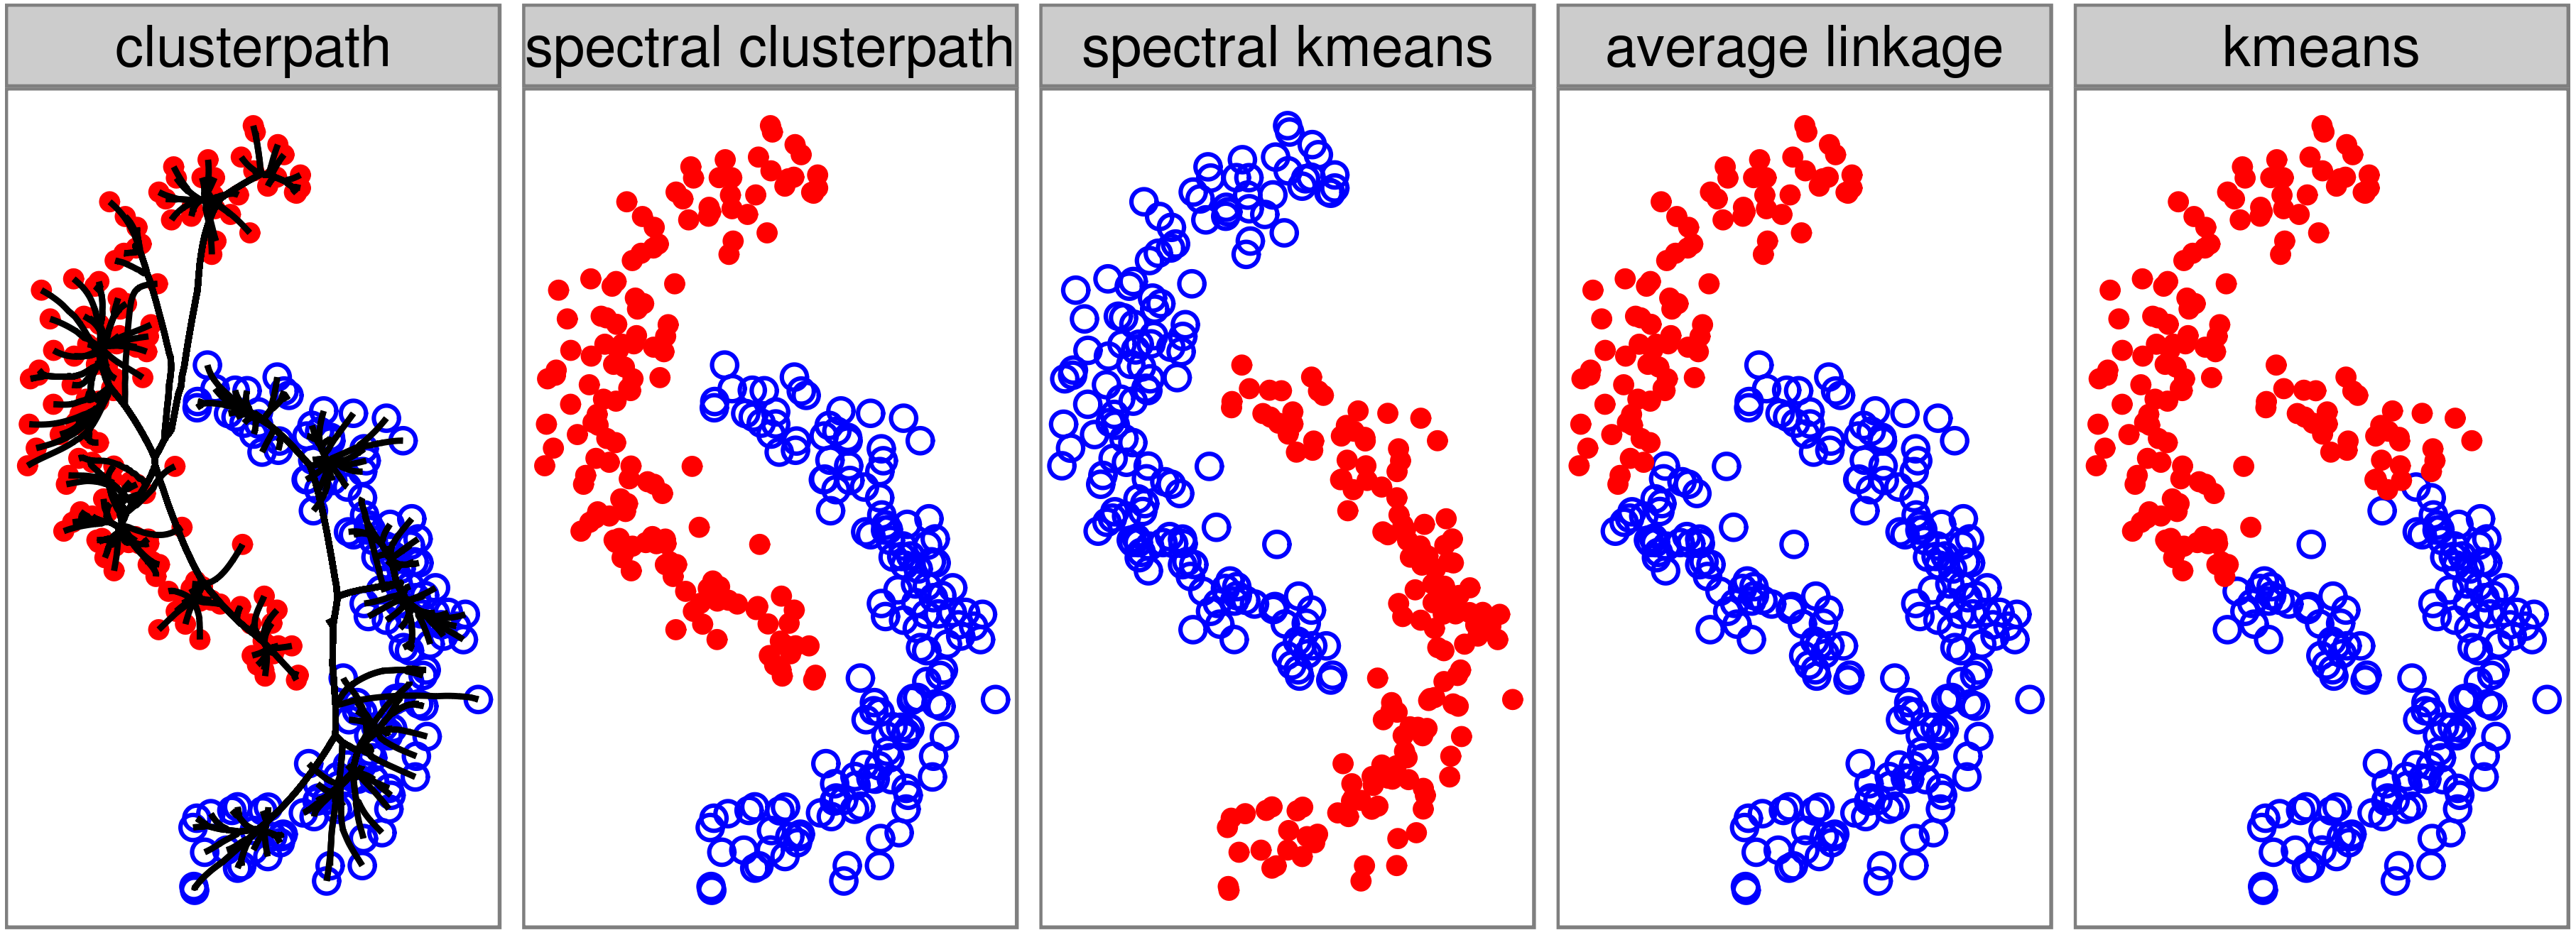
\includegraphics[width=0.3\paperwidth]{moons}

\includegraphics{iris-clusterpath}
{\small
% Created by tikzDevice version 0.5.3 on 2011-05-02 14:31:11
\begin{tikzpicture}[x=1pt,y=1pt]
\draw[color=white,opacity=0] (0,0) rectangle (289.08,361.35);
\begin{scope}
\path[clip] (  0.00,  0.00) rectangle (289.08,361.35);
\end{scope}
\begin{scope}
\path[clip] (  0.00,  0.00) rectangle (289.08,361.35);
\end{scope}
\begin{scope}
\path[clip] (  0.00,  0.00) rectangle (289.08,361.35);
\end{scope}
\begin{scope}
\path[clip] (  0.00,  0.00) rectangle (289.08,361.35);
\end{scope}
\begin{scope}
\path[clip] (  0.00,  0.00) rectangle (289.08,361.35);
\end{scope}
\begin{scope}
\path[clip] (  0.00,  0.00) rectangle (289.08,361.35);
\end{scope}
\begin{scope}
\path[clip] (  0.00,  0.00) rectangle (289.08,361.35);
\end{scope}
\begin{scope}
\path[clip] (  0.00,  0.00) rectangle (289.08,361.35);
\end{scope}
\begin{scope}
\path[clip] (  0.00,  0.00) rectangle (289.08,361.35);
\end{scope}
\begin{scope}
\path[clip] (  0.00,  0.00) rectangle (289.08,361.35);
\end{scope}
\begin{scope}
\path[clip] (  0.00,  0.00) rectangle (289.08,361.35);
\end{scope}
\begin{scope}
\path[clip] (  0.00,  0.00) rectangle (289.08,361.35);
\end{scope}
\begin{scope}
\path[clip] (  0.00,  0.00) rectangle (289.08,361.35);
\end{scope}
\begin{scope}
\path[clip] (  0.00,  0.00) rectangle (289.08,361.35);
\end{scope}
\begin{scope}
\path[clip] (  0.00,  0.00) rectangle (289.08,361.35);
\end{scope}
\begin{scope}
\path[clip] (  0.00,  0.00) rectangle (289.08,361.35);
\end{scope}
\begin{scope}
\path[clip] (  0.00,  0.00) rectangle (289.08,361.35);
\end{scope}
\begin{scope}
\path[clip] (  0.00,  0.00) rectangle (289.08,361.35);
\end{scope}
\begin{scope}
\path[clip] (  0.00,  0.00) rectangle (289.08,361.35);
\end{scope}
\begin{scope}
\path[clip] (  0.00,  0.00) rectangle (289.08,361.35);
\end{scope}
\begin{scope}
\path[clip] (  0.00,  0.00) rectangle (289.08,361.35);

\draw[fill opacity=0.00,draw opacity=0.00,] (  0.00,  0.00) rectangle (289.08,361.35);
\end{scope}
\begin{scope}
\path[clip] (  0.00,  0.00) rectangle (289.08,361.35);
\end{scope}
\begin{scope}
\path[clip] (  0.00,  0.00) rectangle (289.08,361.35);
\end{scope}
\begin{scope}
\path[clip] (  0.00,  0.00) rectangle (289.08,361.35);
\end{scope}
\begin{scope}
\path[clip] (  0.00,  0.00) rectangle (289.08,361.35);
\end{scope}
\begin{scope}
\path[clip] (  0.00,  0.00) rectangle (289.08,361.35);
\end{scope}
\begin{scope}
\path[clip] (  0.00,  0.00) rectangle (289.08,361.35);
\definecolor[named]{drawColor}{rgb}{0.00,0.00,0.00}

\node[color=drawColor,anchor=base,inner sep=0pt, outer sep=0pt, scale=  1.00] at (112.89, 14.45) {Number of clusters%
};
\end{scope}
\begin{scope}
\path[clip] (  0.00,  0.00) rectangle (289.08,361.35);
\end{scope}
\begin{scope}
\path[clip] (  0.00,  0.00) rectangle (289.08,361.35);
\end{scope}
\begin{scope}
\path[clip] (  0.00,  0.00) rectangle (289.08,361.35);
\definecolor[named]{drawColor}{rgb}{0.00,0.00,0.00}

\node[rotate= 90.00,color=drawColor,anchor=base,inner sep=0pt, outer sep=0pt, scale=  1.00] at ( 19.11,184.81) {Normalized Rand index (bigger means better agreement with known clusters)%
};
\end{scope}
\begin{scope}
\path[clip] (  0.00,  0.00) rectangle (289.08,361.35);
\end{scope}
\begin{scope}
\path[clip] (  0.00,  0.00) rectangle (289.08,361.35);
\end{scope}
\begin{scope}
\path[clip] (  0.00,  0.00) rectangle (289.08,361.35);
\end{scope}
\begin{scope}
\path[clip] ( 22.72,346.90) rectangle ( 46.29,346.90);
\end{scope}
\begin{scope}
\path[clip] (  0.00,  0.00) rectangle (289.08,361.35);
\end{scope}
\begin{scope}
\path[clip] ( 22.72,346.90) rectangle ( 46.29,346.90);
\end{scope}
\begin{scope}
\path[clip] (  0.00,  0.00) rectangle (289.08,361.35);
\end{scope}
\begin{scope}
\path[clip] (  0.00,  0.00) rectangle (289.08,361.35);
\end{scope}
\begin{scope}
\path[clip] (  0.00,  0.00) rectangle (289.08,361.35);
\end{scope}
\begin{scope}
\path[clip] ( 22.72,192.09) rectangle ( 46.29,195.70);
\end{scope}
\begin{scope}
\path[clip] (  0.00,  0.00) rectangle (289.08,361.35);
\end{scope}
\begin{scope}
\path[clip] (  0.00,  0.00) rectangle (289.08,361.35);
\end{scope}
\begin{scope}
\path[clip] (  0.00,  0.00) rectangle (289.08,361.35);
\end{scope}
\begin{scope}
\path[clip] ( 22.72, 40.89) rectangle ( 46.29, 40.89);
\end{scope}
\begin{scope}
\path[clip] (  0.00,  0.00) rectangle (289.08,361.35);
\end{scope}
\begin{scope}
\path[clip] ( 22.72, 22.72) rectangle ( 46.29, 40.89);
\end{scope}
\begin{scope}
\path[clip] (  0.00,  0.00) rectangle (289.08,361.35);
\end{scope}
\begin{scope}
\path[clip] ( 22.72, 22.72) rectangle ( 46.29, 22.72);
\end{scope}
\begin{scope}
\path[clip] (  0.00,  0.00) rectangle (289.08,361.35);
\end{scope}
\begin{scope}
\path[clip] ( 46.29,346.90) rectangle ( 46.29,346.90);
\end{scope}
\begin{scope}
\path[clip] (  0.00,  0.00) rectangle (289.08,361.35);
\end{scope}
\begin{scope}
\path[clip] ( 46.29,346.90) rectangle ( 46.29,346.90);
\end{scope}
\begin{scope}
\path[clip] (  0.00,  0.00) rectangle (289.08,361.35);
\end{scope}
\begin{scope}
\path[clip] ( 46.29,195.70) rectangle ( 46.29,346.90);
\end{scope}
\begin{scope}
\path[clip] (  0.00,  0.00) rectangle (289.08,361.35);
\end{scope}
\begin{scope}
\path[clip] ( 46.29,192.09) rectangle ( 46.29,195.70);
\end{scope}
\begin{scope}
\path[clip] (  0.00,  0.00) rectangle (289.08,361.35);
\end{scope}
\begin{scope}
\path[clip] ( 46.29, 40.89) rectangle ( 46.29,192.09);
\end{scope}
\begin{scope}
\path[clip] (  0.00,  0.00) rectangle (289.08,361.35);
\end{scope}
\begin{scope}
\path[clip] ( 46.29, 40.89) rectangle ( 46.29, 40.89);
\end{scope}
\begin{scope}
\path[clip] (  0.00,  0.00) rectangle (289.08,361.35);
\end{scope}
\begin{scope}
\path[clip] ( 46.29, 22.72) rectangle ( 46.29, 40.89);
\end{scope}
\begin{scope}
\path[clip] (  0.00,  0.00) rectangle (289.08,361.35);
\end{scope}
\begin{scope}
\path[clip] ( 46.29, 22.72) rectangle ( 46.29, 22.72);
\end{scope}
\begin{scope}
\path[clip] (  0.00,  0.00) rectangle (289.08,361.35);
\end{scope}
\begin{scope}
\path[clip] ( 46.29,346.90) rectangle (189.23,346.90);
\end{scope}
\begin{scope}
\path[clip] (  0.00,  0.00) rectangle (289.08,361.35);
\end{scope}
\begin{scope}
\path[clip] ( 46.29,346.90) rectangle (189.23,346.90);
\end{scope}
\begin{scope}
\path[clip] (  0.00,  0.00) rectangle (289.08,361.35);
\end{scope}
\begin{scope}
\path[clip] ( 46.29,195.70) rectangle (189.23,346.90);
\end{scope}
\begin{scope}
\path[clip] (  0.00,  0.00) rectangle (289.08,361.35);
\end{scope}
\begin{scope}
\path[clip] ( 46.29,192.09) rectangle (189.23,195.70);
\end{scope}
\begin{scope}
\path[clip] (  0.00,  0.00) rectangle (289.08,361.35);
\end{scope}
\begin{scope}
\path[clip] ( 46.29, 40.89) rectangle (189.23,192.09);
\end{scope}
\begin{scope}
\path[clip] (  0.00,  0.00) rectangle (289.08,361.35);
\end{scope}
\begin{scope}
\path[clip] ( 46.29, 40.89) rectangle (189.23, 40.89);
\end{scope}
\begin{scope}
\path[clip] (  0.00,  0.00) rectangle (289.08,361.35);
\end{scope}
\begin{scope}
\path[clip] (  0.00,  0.00) rectangle (289.08,361.35);
\end{scope}
\begin{scope}
\path[clip] (  0.00,  0.00) rectangle (289.08,361.35);
\end{scope}
\begin{scope}
\path[clip] ( 46.29, 22.72) rectangle (189.23, 22.72);
\end{scope}
\begin{scope}
\path[clip] (  0.00,  0.00) rectangle (289.08,361.35);
\end{scope}
\begin{scope}
\path[clip] (189.23,346.90) rectangle (189.23,346.90);
\end{scope}
\begin{scope}
\path[clip] (  0.00,  0.00) rectangle (289.08,361.35);
\end{scope}
\begin{scope}
\path[clip] (189.23,346.90) rectangle (189.23,346.90);
\end{scope}
\begin{scope}
\path[clip] (  0.00,  0.00) rectangle (289.08,361.35);
\end{scope}
\begin{scope}
\path[clip] (189.23,195.70) rectangle (189.23,346.90);
\end{scope}
\begin{scope}
\path[clip] (  0.00,  0.00) rectangle (289.08,361.35);
\end{scope}
\begin{scope}
\path[clip] (189.23,192.09) rectangle (189.23,195.70);
\end{scope}
\begin{scope}
\path[clip] (  0.00,  0.00) rectangle (289.08,361.35);
\end{scope}
\begin{scope}
\path[clip] (189.23, 40.89) rectangle (189.23,192.09);
\end{scope}
\begin{scope}
\path[clip] (  0.00,  0.00) rectangle (289.08,361.35);
\end{scope}
\begin{scope}
\path[clip] (189.23, 40.89) rectangle (189.23, 40.89);
\end{scope}
\begin{scope}
\path[clip] (  0.00,  0.00) rectangle (289.08,361.35);
\end{scope}
\begin{scope}
\path[clip] (189.23, 22.72) rectangle (189.23, 40.89);
\end{scope}
\begin{scope}
\path[clip] (  0.00,  0.00) rectangle (289.08,361.35);
\end{scope}
\begin{scope}
\path[clip] (189.23, 22.72) rectangle (189.23, 22.72);
\end{scope}
\begin{scope}
\path[clip] (  0.00,  0.00) rectangle (289.08,361.35);
\end{scope}
\begin{scope}
\path[clip] (189.23,346.90) rectangle (203.07,346.90);
\end{scope}
\begin{scope}
\path[clip] (  0.00,  0.00) rectangle (289.08,361.35);
\end{scope}
\begin{scope}
\path[clip] (189.23,346.90) rectangle (203.07,346.90);
\end{scope}
\begin{scope}
\path[clip] (  0.00,  0.00) rectangle (289.08,361.35);
\end{scope}
\begin{scope}
\path[clip] (189.23,195.70) rectangle (203.07,346.90);
\end{scope}
\begin{scope}
\path[clip] (  0.00,  0.00) rectangle (289.08,361.35);
\end{scope}
\begin{scope}
\path[clip] (189.23,192.09) rectangle (203.07,195.70);
\end{scope}
\begin{scope}
\path[clip] (  0.00,  0.00) rectangle (289.08,361.35);
\end{scope}
\begin{scope}
\path[clip] (189.23, 40.89) rectangle (203.07,192.09);
\end{scope}
\begin{scope}
\path[clip] (  0.00,  0.00) rectangle (289.08,361.35);
\end{scope}
\begin{scope}
\path[clip] (189.23, 40.89) rectangle (203.07, 40.89);
\end{scope}
\begin{scope}
\path[clip] (  0.00,  0.00) rectangle (289.08,361.35);
\end{scope}
\begin{scope}
\path[clip] (189.23, 22.72) rectangle (203.07, 40.89);
\end{scope}
\begin{scope}
\path[clip] (  0.00,  0.00) rectangle (289.08,361.35);
\end{scope}
\begin{scope}
\path[clip] (189.23, 22.72) rectangle (203.07, 22.72);
\end{scope}
\begin{scope}
\path[clip] (  0.00,  0.00) rectangle (289.08,361.35);
\end{scope}
\begin{scope}
\path[clip] (203.07,346.90) rectangle (203.07,346.90);
\end{scope}
\begin{scope}
\path[clip] (  0.00,  0.00) rectangle (289.08,361.35);
\end{scope}
\begin{scope}
\path[clip] (203.07,346.90) rectangle (203.07,346.90);
\end{scope}
\begin{scope}
\path[clip] (  0.00,  0.00) rectangle (289.08,361.35);
\end{scope}
\begin{scope}
\path[clip] (203.07,195.70) rectangle (203.07,346.90);
\end{scope}
\begin{scope}
\path[clip] (  0.00,  0.00) rectangle (289.08,361.35);
\end{scope}
\begin{scope}
\path[clip] (203.07,192.09) rectangle (203.07,195.70);
\end{scope}
\begin{scope}
\path[clip] (  0.00,  0.00) rectangle (289.08,361.35);
\end{scope}
\begin{scope}
\path[clip] (203.07, 40.89) rectangle (203.07,192.09);
\end{scope}
\begin{scope}
\path[clip] (  0.00,  0.00) rectangle (289.08,361.35);
\end{scope}
\begin{scope}
\path[clip] (203.07, 40.89) rectangle (203.07, 40.89);
\end{scope}
\begin{scope}
\path[clip] (  0.00,  0.00) rectangle (289.08,361.35);
\end{scope}
\begin{scope}
\path[clip] (203.07, 22.72) rectangle (203.07, 40.89);
\end{scope}
\begin{scope}
\path[clip] (  0.00,  0.00) rectangle (289.08,361.35);
\end{scope}
\begin{scope}
\path[clip] (203.07, 22.72) rectangle (203.07, 22.72);
\end{scope}
\begin{scope}
\path[clip] (  0.00,  0.00) rectangle (289.08,361.35);
\end{scope}
\begin{scope}
\path[clip] ( 22.72,346.90) rectangle ( 46.29,346.90);
\end{scope}
\begin{scope}
\path[clip] (  0.00,  0.00) rectangle (289.08,361.35);
\end{scope}
\begin{scope}
\path[clip] ( 22.72,346.90) rectangle ( 46.29,346.90);
\end{scope}
\begin{scope}
\path[clip] (  0.00,  0.00) rectangle (289.08,361.35);
\end{scope}
\begin{scope}
\path[clip] (  0.00,  0.00) rectangle (289.08,361.35);
\definecolor[named]{drawColor}{rgb}{0.00,0.00,0.00}

\draw[color=drawColor,line width= 0.0pt,line cap=round,line join=round,fill opacity=0.00,] ( 41.95,233.50) -- ( 46.29,233.50);

\draw[color=drawColor,line width= 0.0pt,line cap=round,line join=round,fill opacity=0.00,] ( 41.95,271.30) -- ( 46.29,271.30);

\draw[color=drawColor,line width= 0.0pt,line cap=round,line join=round,fill opacity=0.00,] ( 41.95,309.10) -- ( 46.29,309.10);

\draw[color=drawColor,line width= 0.0pt,line cap=round,line join=round,fill opacity=0.00,] ( 41.95,346.90) -- ( 46.29,346.90);

\node[color=drawColor,anchor=base east,inner sep=0pt, outer sep=0pt, scale=  0.80] at ( 39.35,230.19) {0.4%
};

\node[color=drawColor,anchor=base east,inner sep=0pt, outer sep=0pt, scale=  0.80] at ( 39.35,267.99) {0.6%
};

\node[color=drawColor,anchor=base east,inner sep=0pt, outer sep=0pt, scale=  0.80] at ( 39.35,305.79) {0.8%
};

\node[color=drawColor,anchor=base east,inner sep=0pt, outer sep=0pt, scale=  0.80] at ( 39.35,343.59) {1.0%
};
\end{scope}
\begin{scope}
\path[clip] (  0.00,  0.00) rectangle (289.08,361.35);
\end{scope}
\begin{scope}
\path[clip] ( 22.72,192.09) rectangle ( 46.29,195.70);
\end{scope}
\begin{scope}
\path[clip] (  0.00,  0.00) rectangle (289.08,361.35);
\end{scope}
\begin{scope}
\path[clip] (  0.00,  0.00) rectangle (289.08,361.35);
\definecolor[named]{drawColor}{rgb}{0.00,0.00,0.00}

\draw[color=drawColor,line width= 0.0pt,line cap=round,line join=round,fill opacity=0.00,] ( 41.95, 78.69) -- ( 46.29, 78.69);

\draw[color=drawColor,line width= 0.0pt,line cap=round,line join=round,fill opacity=0.00,] ( 41.95,116.49) -- ( 46.29,116.49);

\draw[color=drawColor,line width= 0.0pt,line cap=round,line join=round,fill opacity=0.00,] ( 41.95,154.29) -- ( 46.29,154.29);

\draw[color=drawColor,line width= 0.0pt,line cap=round,line join=round,fill opacity=0.00,] ( 41.95,192.09) -- ( 46.29,192.09);

\node[color=drawColor,anchor=base east,inner sep=0pt, outer sep=0pt, scale=  0.80] at ( 39.35, 75.39) {0.4%
};

\node[color=drawColor,anchor=base east,inner sep=0pt, outer sep=0pt, scale=  0.80] at ( 39.35,113.18) {0.6%
};

\node[color=drawColor,anchor=base east,inner sep=0pt, outer sep=0pt, scale=  0.80] at ( 39.35,150.98) {0.8%
};

\node[color=drawColor,anchor=base east,inner sep=0pt, outer sep=0pt, scale=  0.80] at ( 39.35,188.78) {1.0%
};
\end{scope}
\begin{scope}
\path[clip] (  0.00,  0.00) rectangle (289.08,361.35);
\end{scope}
\begin{scope}
\path[clip] ( 22.72, 40.89) rectangle ( 46.29, 40.89);
\end{scope}
\begin{scope}
\path[clip] (  0.00,  0.00) rectangle (289.08,361.35);
\end{scope}
\begin{scope}
\path[clip] ( 22.72, 22.72) rectangle ( 46.29, 40.89);
\end{scope}
\begin{scope}
\path[clip] (  0.00,  0.00) rectangle (289.08,361.35);
\end{scope}
\begin{scope}
\path[clip] ( 22.72, 22.72) rectangle ( 46.29, 22.72);
\end{scope}
\begin{scope}
\path[clip] (  0.00,  0.00) rectangle (289.08,361.35);
\end{scope}
\begin{scope}
\path[clip] ( 46.29,346.90) rectangle ( 46.29,346.90);
\end{scope}
\begin{scope}
\path[clip] (  0.00,  0.00) rectangle (289.08,361.35);
\end{scope}
\begin{scope}
\path[clip] ( 46.29,346.90) rectangle ( 46.29,346.90);
\end{scope}
\begin{scope}
\path[clip] (  0.00,  0.00) rectangle (289.08,361.35);
\end{scope}
\begin{scope}
\path[clip] ( 46.29,195.70) rectangle ( 46.29,346.90);
\end{scope}
\begin{scope}
\path[clip] (  0.00,  0.00) rectangle (289.08,361.35);
\end{scope}
\begin{scope}
\path[clip] ( 46.29,192.09) rectangle ( 46.29,195.70);
\end{scope}
\begin{scope}
\path[clip] (  0.00,  0.00) rectangle (289.08,361.35);
\end{scope}
\begin{scope}
\path[clip] ( 46.29, 40.89) rectangle ( 46.29,192.09);
\end{scope}
\begin{scope}
\path[clip] (  0.00,  0.00) rectangle (289.08,361.35);
\end{scope}
\begin{scope}
\path[clip] ( 46.29, 40.89) rectangle ( 46.29, 40.89);
\end{scope}
\begin{scope}
\path[clip] (  0.00,  0.00) rectangle (289.08,361.35);
\end{scope}
\begin{scope}
\path[clip] ( 46.29, 22.72) rectangle ( 46.29, 40.89);
\end{scope}
\begin{scope}
\path[clip] (  0.00,  0.00) rectangle (289.08,361.35);
\end{scope}
\begin{scope}
\path[clip] ( 46.29, 22.72) rectangle ( 46.29, 22.72);
\end{scope}
\begin{scope}
\path[clip] (  0.00,  0.00) rectangle (289.08,361.35);
\end{scope}
\begin{scope}
\path[clip] ( 46.29,346.90) rectangle (189.23,346.90);
\end{scope}
\begin{scope}
\path[clip] (  0.00,  0.00) rectangle (289.08,361.35);
\end{scope}
\begin{scope}
\path[clip] ( 46.29,346.90) rectangle (189.23,346.90);
\end{scope}
\begin{scope}
\path[clip] (  0.00,  0.00) rectangle (289.08,361.35);
\end{scope}
\begin{scope}
\path[clip] ( 46.29,195.70) rectangle (189.23,346.90);
\definecolor[named]{fillColor}{rgb}{1.00,1.00,1.00}

\draw[fill=fillColor,draw opacity=0.00,] ( 46.29,195.70) rectangle (189.23,346.90);
\definecolor[named]{drawColor}{rgb}{0.98,0.98,0.98}

\draw[color=drawColor,line cap=round,line join=round,fill opacity=0.00,] ( 46.29,195.70) --
	(189.23,195.70);

\draw[color=drawColor,line cap=round,line join=round,fill opacity=0.00,] ( 46.29,214.60) --
	(189.23,214.60);

\draw[color=drawColor,line cap=round,line join=round,fill opacity=0.00,] ( 46.29,233.50) --
	(189.23,233.50);

\draw[color=drawColor,line cap=round,line join=round,fill opacity=0.00,] ( 46.29,252.40) --
	(189.23,252.40);

\draw[color=drawColor,line cap=round,line join=round,fill opacity=0.00,] ( 46.29,271.30) --
	(189.23,271.30);

\draw[color=drawColor,line cap=round,line join=round,fill opacity=0.00,] ( 46.29,290.20) --
	(189.23,290.20);

\draw[color=drawColor,line cap=round,line join=round,fill opacity=0.00,] ( 46.29,309.10) --
	(189.23,309.10);

\draw[color=drawColor,line cap=round,line join=round,fill opacity=0.00,] ( 46.29,328.00) --
	(189.23,328.00);

\draw[color=drawColor,line cap=round,line join=round,fill opacity=0.00,] ( 46.29,346.90) --
	(189.23,346.90);

\draw[color=drawColor,line cap=round,line join=round,fill opacity=0.00,] ( 46.29,195.70) --
	( 46.29,346.90);

\draw[color=drawColor,line cap=round,line join=round,fill opacity=0.00,] ( 54.23,195.70) --
	( 54.23,346.90);

\draw[color=drawColor,line cap=round,line join=round,fill opacity=0.00,] ( 62.17,195.70) --
	( 62.17,346.90);

\draw[color=drawColor,line cap=round,line join=round,fill opacity=0.00,] ( 78.05,195.70) --
	( 78.05,346.90);

\draw[color=drawColor,line cap=round,line join=round,fill opacity=0.00,] ( 93.94,195.70) --
	( 93.94,346.90);

\draw[color=drawColor,line cap=round,line join=round,fill opacity=0.00,] (133.64,195.70) --
	(133.64,346.90);

\draw[color=drawColor,line cap=round,line join=round,fill opacity=0.00,] (173.35,195.70) --
	(173.35,346.90);
\definecolor[named]{drawColor}{rgb}{0.90,0.90,0.90}

\draw[color=drawColor,line width= 0.0pt,line cap=round,line join=round,fill opacity=0.00,] ( 46.29,233.50) --
	(189.23,233.50);

\draw[color=drawColor,line width= 0.0pt,line cap=round,line join=round,fill opacity=0.00,] ( 46.29,271.30) --
	(189.23,271.30);

\draw[color=drawColor,line width= 0.0pt,line cap=round,line join=round,fill opacity=0.00,] ( 46.29,309.10) --
	(189.23,309.10);

\draw[color=drawColor,line width= 0.0pt,line cap=round,line join=round,fill opacity=0.00,] ( 46.29,346.90) --
	(189.23,346.90);

\draw[color=drawColor,line width= 0.0pt,line cap=round,line join=round,fill opacity=0.00,] ( 46.29,195.70) --
	( 46.29,346.90);

\draw[color=drawColor,line width= 0.0pt,line cap=round,line join=round,fill opacity=0.00,] ( 62.17,195.70) --
	( 62.17,346.90);

\draw[color=drawColor,line width= 0.0pt,line cap=round,line join=round,fill opacity=0.00,] ( 93.94,195.70) --
	( 93.94,346.90);

\draw[color=drawColor,line width= 0.0pt,line cap=round,line join=round,fill opacity=0.00,] (173.35,195.70) --
	(173.35,346.90);
\definecolor[named]{drawColor}{rgb}{0.97,0.46,0.43}

\draw[color=drawColor,line width= 2.0pt,line join=round,fill opacity=0.00,] ( 46.29,265.27) --
	( 62.17,263.43) --
	( 78.05,262.27) --
	( 93.94,262.19) --
	(109.82,261.83) --
	(125.70,261.23) --
	(141.58,259.77) --
	(157.46,257.96) --
	(173.35,255.95) --
	(189.23,255.65);
\definecolor[named]{drawColor}{rgb}{0.72,0.62,0.00}

\draw[color=drawColor,line width= 2.0pt,dash pattern=on 2pt off 2pt ,line join=round,fill opacity=0.00,] ( 46.29,265.27) --
	( 62.17,263.43) --
	( 78.05,262.58) --
	( 93.94,260.74) --
	(109.82,260.20) --
	(125.70,259.77) --
	(141.58,259.36) --
	(157.46,259.32) --
	(173.35,258.24) --
	(189.23,256.37);
\definecolor[named]{drawColor}{rgb}{0.00,0.73,0.22}

\draw[color=drawColor,line width= 2.0pt,dash pattern=on 4pt off 2pt ,line join=round,fill opacity=0.00,] ( 46.29,265.27) --
	( 62.17,263.43) --
	( 78.05,262.58) --
	( 93.94,262.19) --
	(109.82,261.63) --
	(125.70,259.77) --
	(141.58,259.36) --
	(157.46,258.47) --
	(173.35,258.03) --
	(189.23,255.63);
\definecolor[named]{drawColor}{rgb}{0.00,0.75,0.77}

\draw[color=drawColor,line width= 2.0pt,dash pattern=on 4pt off 4pt ,line join=round,fill opacity=0.00,] ( 46.29,265.27) --
	( 62.17,328.73) --
	( 78.05,243.42) --
	( 93.94,305.57) --
	(109.82,281.69) --
	(125.70,270.95) --
	(141.58,250.13) --
	(157.46,237.41) --
	(173.35,232.85) --
	(189.23,231.46);
\definecolor[named]{drawColor}{rgb}{0.38,0.61,1.00}

\draw[color=drawColor,line width= 2.0pt,dash pattern=on 1pt off 3pt ,line join=round,fill opacity=0.00,] ( 46.29,265.27) --
	( 62.17,264.14) --
	( 78.05,262.27) --
	( 93.94,262.02) --
	(109.82,254.27) --
	(125.70,262.55) --
	(141.58,254.36) --
	(157.46,252.62) --
	(173.35,228.34) --
	(189.23,234.05);
\definecolor[named]{drawColor}{rgb}{0.96,0.39,0.89}

\draw[color=drawColor,line width= 2.0pt,dash pattern=on 1pt off 3pt on 4pt off 3pt ,line join=round,fill opacity=0.00,] ( 46.29,265.27) --
	( 62.17,266.69) --
	( 78.05,257.27) --
	( 93.94,248.43) --
	(109.82,240.30) --
	(125.70,235.60) --
	(141.58,232.24) --
	(157.46,227.93) --
	(173.35,223.60) --
	(189.23,220.48);

\draw[color=drawColor,line width= 2.0pt,dash pattern=on 1pt off 3pt on 4pt off 3pt ,line join=round,fill opacity=0.00,] ( 46.29,265.27) -- ( 46.29,265.27);

\draw[color=drawColor,line width= 2.0pt,dash pattern=on 1pt off 3pt on 4pt off 3pt ,line join=round,fill opacity=0.00,] ( 62.17,252.00) -- ( 62.17,281.38);

\draw[color=drawColor,line width= 2.0pt,dash pattern=on 1pt off 3pt on 4pt off 3pt ,line join=round,fill opacity=0.00,] ( 78.05,249.16) -- ( 78.05,265.38);

\draw[color=drawColor,line width= 2.0pt,dash pattern=on 1pt off 3pt on 4pt off 3pt ,line join=round,fill opacity=0.00,] ( 93.94,235.55) -- ( 93.94,261.31);

\draw[color=drawColor,line width= 2.0pt,dash pattern=on 1pt off 3pt on 4pt off 3pt ,line join=round,fill opacity=0.00,] (109.82,226.64) -- (109.82,253.96);

\draw[color=drawColor,line width= 2.0pt,dash pattern=on 1pt off 3pt on 4pt off 3pt ,line join=round,fill opacity=0.00,] (125.70,220.21) -- (125.70,250.99);

\draw[color=drawColor,line width= 2.0pt,dash pattern=on 1pt off 3pt on 4pt off 3pt ,line join=round,fill opacity=0.00,] (141.58,216.87) -- (141.58,247.60);

\draw[color=drawColor,line width= 2.0pt,dash pattern=on 1pt off 3pt on 4pt off 3pt ,line join=round,fill opacity=0.00,] (157.46,213.94) -- (157.46,241.91);

\draw[color=drawColor,line width= 2.0pt,dash pattern=on 1pt off 3pt on 4pt off 3pt ,line join=round,fill opacity=0.00,] (173.35,211.10) -- (173.35,236.10);

\draw[color=drawColor,line width= 2.0pt,dash pattern=on 1pt off 3pt on 4pt off 3pt ,line join=round,fill opacity=0.00,] (189.23,208.57) -- (189.23,232.39);
\definecolor[named]{drawColor}{rgb}{0.50,0.50,0.50}

\draw[color=drawColor,line cap=round,line join=round,fill opacity=0.00,] ( 46.29,195.70) rectangle (189.23,346.90);
\end{scope}
\begin{scope}
\path[clip] (  0.00,  0.00) rectangle (289.08,361.35);
\end{scope}
\begin{scope}
\path[clip] ( 46.29,192.09) rectangle (189.23,195.70);
\end{scope}
\begin{scope}
\path[clip] (  0.00,  0.00) rectangle (289.08,361.35);
\end{scope}
\begin{scope}
\path[clip] ( 46.29, 40.89) rectangle (189.23,192.09);
\definecolor[named]{fillColor}{rgb}{1.00,1.00,1.00}

\draw[fill=fillColor,draw opacity=0.00,] ( 46.29, 40.89) rectangle (189.23,192.09);
\definecolor[named]{drawColor}{rgb}{0.98,0.98,0.98}

\draw[color=drawColor,line cap=round,line join=round,fill opacity=0.00,] ( 46.29, 40.89) --
	(189.23, 40.89);

\draw[color=drawColor,line cap=round,line join=round,fill opacity=0.00,] ( 46.29, 59.79) --
	(189.23, 59.79);

\draw[color=drawColor,line cap=round,line join=round,fill opacity=0.00,] ( 46.29, 78.69) --
	(189.23, 78.69);

\draw[color=drawColor,line cap=round,line join=round,fill opacity=0.00,] ( 46.29, 97.59) --
	(189.23, 97.59);

\draw[color=drawColor,line cap=round,line join=round,fill opacity=0.00,] ( 46.29,116.49) --
	(189.23,116.49);

\draw[color=drawColor,line cap=round,line join=round,fill opacity=0.00,] ( 46.29,135.39) --
	(189.23,135.39);

\draw[color=drawColor,line cap=round,line join=round,fill opacity=0.00,] ( 46.29,154.29) --
	(189.23,154.29);

\draw[color=drawColor,line cap=round,line join=round,fill opacity=0.00,] ( 46.29,173.19) --
	(189.23,173.19);

\draw[color=drawColor,line cap=round,line join=round,fill opacity=0.00,] ( 46.29,192.09) --
	(189.23,192.09);

\draw[color=drawColor,line cap=round,line join=round,fill opacity=0.00,] ( 46.29, 40.89) --
	( 46.29,192.09);

\draw[color=drawColor,line cap=round,line join=round,fill opacity=0.00,] ( 54.23, 40.89) --
	( 54.23,192.09);

\draw[color=drawColor,line cap=round,line join=round,fill opacity=0.00,] ( 62.17, 40.89) --
	( 62.17,192.09);

\draw[color=drawColor,line cap=round,line join=round,fill opacity=0.00,] ( 78.05, 40.89) --
	( 78.05,192.09);

\draw[color=drawColor,line cap=round,line join=round,fill opacity=0.00,] ( 93.94, 40.89) --
	( 93.94,192.09);

\draw[color=drawColor,line cap=round,line join=round,fill opacity=0.00,] (133.64, 40.89) --
	(133.64,192.09);

\draw[color=drawColor,line cap=round,line join=round,fill opacity=0.00,] (173.35, 40.89) --
	(173.35,192.09);
\definecolor[named]{drawColor}{rgb}{0.90,0.90,0.90}

\draw[color=drawColor,line width= 0.0pt,line cap=round,line join=round,fill opacity=0.00,] ( 46.29, 78.69) --
	(189.23, 78.69);

\draw[color=drawColor,line width= 0.0pt,line cap=round,line join=round,fill opacity=0.00,] ( 46.29,116.49) --
	(189.23,116.49);

\draw[color=drawColor,line width= 0.0pt,line cap=round,line join=round,fill opacity=0.00,] ( 46.29,154.29) --
	(189.23,154.29);

\draw[color=drawColor,line width= 0.0pt,line cap=round,line join=round,fill opacity=0.00,] ( 46.29,192.09) --
	(189.23,192.09);

\draw[color=drawColor,line width= 0.0pt,line cap=round,line join=round,fill opacity=0.00,] ( 46.29, 40.89) --
	( 46.29,192.09);

\draw[color=drawColor,line width= 0.0pt,line cap=round,line join=round,fill opacity=0.00,] ( 62.17, 40.89) --
	( 62.17,192.09);

\draw[color=drawColor,line width= 0.0pt,line cap=round,line join=round,fill opacity=0.00,] ( 93.94, 40.89) --
	( 93.94,192.09);

\draw[color=drawColor,line width= 0.0pt,line cap=round,line join=round,fill opacity=0.00,] (173.35, 40.89) --
	(173.35,192.09);
\definecolor[named]{drawColor}{rgb}{0.97,0.46,0.43}

\draw[color=drawColor,line width= 2.0pt,line join=round,fill opacity=0.00,] ( 46.29,192.09) --
	( 62.17,190.83) --
	( 78.05,189.58) --
	( 93.94,158.73) --
	(109.82,136.95) --
	(125.70,120.07) --
	(141.58, 94.51) --
	(157.46, 94.21) --
	(173.35, 64.83) --
	(189.23, 61.58);
\definecolor[named]{drawColor}{rgb}{0.72,0.62,0.00}

\draw[color=drawColor,line width= 2.0pt,dash pattern=on 2pt off 2pt ,line join=round,fill opacity=0.00,] ( 46.29, 13.73) --
	( 62.17,144.42) --
	( 78.05,132.64) --
	( 93.94,131.87) --
	(109.82,131.65) --
	(125.70,122.97) --
	(141.58, 79.28) --
	(157.46, 79.27) --
	(173.35, 67.35);
\definecolor[named]{drawColor}{rgb}{0.00,0.73,0.22}

\draw[color=drawColor,line width= 2.0pt,dash pattern=on 4pt off 2pt ,line join=round,fill opacity=0.00,] ( 46.29,192.09) --
	( 62.17,160.98) --
	( 78.05,154.36) --
	( 93.94,107.16) --
	(109.82, 93.34) --
	(125.70, 67.83) --
	(141.58, 58.38) --
	(157.46, 56.71) --
	(173.35, 56.69) --
	(189.23, 56.39);
\definecolor[named]{drawColor}{rgb}{0.00,0.75,0.77}

\draw[color=drawColor,line width= 2.0pt,dash pattern=on 4pt off 4pt ,line join=round,fill opacity=0.00,] ( 46.29,106.30) --
	( 62.17, 45.06) --
	( 78.05, 96.26) --
	( 93.94, 81.92) --
	(109.82, 67.84) --
	(125.70, 57.84) --
	(141.58, 50.45) --
	(157.46, 45.51) --
	(173.35, 44.39) --
	(189.23, 42.52);
\definecolor[named]{drawColor}{rgb}{0.38,0.61,1.00}

\draw[color=drawColor,line width= 2.0pt,dash pattern=on 1pt off 3pt ,line join=round,fill opacity=0.00,] ( 46.29, 66.33) --
	( 62.17, 55.66) --
	( 78.05, 98.64) --
	( 93.94, 82.80) --
	(109.82, 68.94) --
	(125.70, 60.65) --
	(141.58, 52.24) --
	(157.46, 49.38) --
	(173.35, 46.18) --
	(189.23, 41.33);
\definecolor[named]{drawColor}{rgb}{0.96,0.39,0.89}

\draw[color=drawColor,line width= 2.0pt,dash pattern=on 1pt off 3pt on 4pt off 3pt ,line join=round,fill opacity=0.00,] ( 46.29, 60.52) --
	( 62.17, 57.67) --
	( 78.05, 58.80) --
	( 93.94, 57.74) --
	(109.82, 56.09) --
	(125.70, 53.06) --
	(141.58, 49.58) --
	(157.46, 45.86) --
	(173.35, 42.11) --
	(189.23, 39.09);

\draw[color=drawColor,line width= 2.0pt,dash pattern=on 1pt off 3pt on 4pt off 3pt ,line join=round,fill opacity=0.00,] ( 46.29, 60.52) -- ( 46.29, 60.52);

\draw[color=drawColor,line width= 2.0pt,dash pattern=on 1pt off 3pt on 4pt off 3pt ,line join=round,fill opacity=0.00,] ( 62.17, 55.96) -- ( 62.17, 59.38);

\draw[color=drawColor,line width= 2.0pt,dash pattern=on 1pt off 3pt on 4pt off 3pt ,line join=round,fill opacity=0.00,] ( 78.05, 56.01) -- ( 78.05, 61.59);

\draw[color=drawColor,line width= 2.0pt,dash pattern=on 1pt off 3pt on 4pt off 3pt ,line join=round,fill opacity=0.00,] ( 93.94, 52.93) -- ( 93.94, 62.56);

\draw[color=drawColor,line width= 2.0pt,dash pattern=on 1pt off 3pt on 4pt off 3pt ,line join=round,fill opacity=0.00,] (109.82, 51.15) -- (109.82, 61.02);

\draw[color=drawColor,line width= 2.0pt,dash pattern=on 1pt off 3pt on 4pt off 3pt ,line join=round,fill opacity=0.00,] (125.70, 49.20) -- (125.70, 56.92);

\draw[color=drawColor,line width= 2.0pt,dash pattern=on 1pt off 3pt on 4pt off 3pt ,line join=round,fill opacity=0.00,] (141.58, 46.63) -- (141.58, 52.54);

\draw[color=drawColor,line width= 2.0pt,dash pattern=on 1pt off 3pt on 4pt off 3pt ,line join=round,fill opacity=0.00,] (157.46, 43.80) -- (157.46, 47.91);

\draw[color=drawColor,line width= 2.0pt,dash pattern=on 1pt off 3pt on 4pt off 3pt ,line join=round,fill opacity=0.00,] (173.35, 41.33) -- (173.35, 42.88);

\draw[color=drawColor,line width= 2.0pt,dash pattern=on 1pt off 3pt on 4pt off 3pt ,line join=round,fill opacity=0.00,] (189.23, 37.64) -- (189.23, 40.53);
\definecolor[named]{drawColor}{rgb}{0.50,0.50,0.50}

\draw[color=drawColor,line cap=round,line join=round,fill opacity=0.00,] ( 46.29, 40.89) rectangle (189.23,192.09);
\end{scope}
\begin{scope}
\path[clip] (  0.00,  0.00) rectangle (289.08,361.35);
\end{scope}
\begin{scope}
\path[clip] ( 46.29, 40.89) rectangle (189.23, 40.89);
\end{scope}
\begin{scope}
\path[clip] (  0.00,  0.00) rectangle (289.08,361.35);
\end{scope}
\begin{scope}
\path[clip] (  0.00,  0.00) rectangle (289.08,361.35);
\definecolor[named]{drawColor}{rgb}{0.00,0.00,0.00}

\draw[color=drawColor,line width= 0.0pt,line cap=round,line join=round,fill opacity=0.00,] ( 46.29, 36.56) -- ( 46.29, 40.89);

\draw[color=drawColor,line width= 0.0pt,line cap=round,line join=round,fill opacity=0.00,] ( 62.17, 36.56) -- ( 62.17, 40.89);

\draw[color=drawColor,line width= 0.0pt,line cap=round,line join=round,fill opacity=0.00,] ( 93.94, 36.56) -- ( 93.94, 40.89);

\draw[color=drawColor,line width= 0.0pt,line cap=round,line join=round,fill opacity=0.00,] (173.35, 36.56) -- (173.35, 40.89);

\node[color=drawColor,anchor=base,inner sep=0pt, outer sep=0pt, scale=  0.80] at ( 46.29, 27.34) {2%
};

\node[color=drawColor,anchor=base,inner sep=0pt, outer sep=0pt, scale=  0.80] at ( 62.17, 27.34) {3%
};

\node[color=drawColor,anchor=base,inner sep=0pt, outer sep=0pt, scale=  0.80] at ( 93.94, 27.34) {5%
};

\node[color=drawColor,anchor=base,inner sep=0pt, outer sep=0pt, scale=  0.80] at (173.35, 27.34) {10%
};
\end{scope}
\begin{scope}
\path[clip] (  0.00,  0.00) rectangle (289.08,361.35);
\end{scope}
\begin{scope}
\path[clip] ( 46.29, 22.72) rectangle (189.23, 22.72);
\end{scope}
\begin{scope}
\path[clip] (  0.00,  0.00) rectangle (289.08,361.35);
\end{scope}
\begin{scope}
\path[clip] (189.23,346.90) rectangle (189.23,346.90);
\end{scope}
\begin{scope}
\path[clip] (  0.00,  0.00) rectangle (289.08,361.35);
\end{scope}
\begin{scope}
\path[clip] (189.23,346.90) rectangle (189.23,346.90);
\end{scope}
\begin{scope}
\path[clip] (  0.00,  0.00) rectangle (289.08,361.35);
\end{scope}
\begin{scope}
\path[clip] (189.23,195.70) rectangle (189.23,346.90);
\end{scope}
\begin{scope}
\path[clip] (  0.00,  0.00) rectangle (289.08,361.35);
\end{scope}
\begin{scope}
\path[clip] (189.23,192.09) rectangle (189.23,195.70);
\end{scope}
\begin{scope}
\path[clip] (  0.00,  0.00) rectangle (289.08,361.35);
\end{scope}
\begin{scope}
\path[clip] (189.23, 40.89) rectangle (189.23,192.09);
\end{scope}
\begin{scope}
\path[clip] (  0.00,  0.00) rectangle (289.08,361.35);
\end{scope}
\begin{scope}
\path[clip] (189.23, 40.89) rectangle (189.23, 40.89);
\end{scope}
\begin{scope}
\path[clip] (  0.00,  0.00) rectangle (289.08,361.35);
\end{scope}
\begin{scope}
\path[clip] (189.23, 22.72) rectangle (189.23, 40.89);
\end{scope}
\begin{scope}
\path[clip] (  0.00,  0.00) rectangle (289.08,361.35);
\end{scope}
\begin{scope}
\path[clip] (189.23, 22.72) rectangle (189.23, 22.72);
\end{scope}
\begin{scope}
\path[clip] (  0.00,  0.00) rectangle (289.08,361.35);
\end{scope}
\begin{scope}
\path[clip] (189.23,346.90) rectangle (203.07,346.90);
\end{scope}
\begin{scope}
\path[clip] (  0.00,  0.00) rectangle (289.08,361.35);
\end{scope}
\begin{scope}
\path[clip] (189.23,346.90) rectangle (203.07,346.90);
\end{scope}
\begin{scope}
\path[clip] (  0.00,  0.00) rectangle (289.08,361.35);
\end{scope}
\begin{scope}
\path[clip] (189.23,195.70) rectangle (203.07,346.90);
\definecolor[named]{drawColor}{rgb}{0.50,0.50,0.50}
\definecolor[named]{fillColor}{rgb}{0.80,0.80,0.80}

\draw[color=drawColor,line cap=round,line join=round,fill=fillColor,] (189.23,195.70) rectangle (203.07,346.90);
\definecolor[named]{drawColor}{rgb}{0.00,0.00,0.00}

\node[rotate=-90.00,color=drawColor,anchor=base,inner sep=0pt, outer sep=0pt, scale=  0.80] at (192.84,271.30) {data: iris%
};
\end{scope}
\begin{scope}
\path[clip] (  0.00,  0.00) rectangle (289.08,361.35);
\end{scope}
\begin{scope}
\path[clip] (189.23,192.09) rectangle (203.07,195.70);
\end{scope}
\begin{scope}
\path[clip] (  0.00,  0.00) rectangle (289.08,361.35);
\end{scope}
\begin{scope}
\path[clip] (189.23, 40.89) rectangle (203.07,192.09);
\definecolor[named]{drawColor}{rgb}{0.50,0.50,0.50}
\definecolor[named]{fillColor}{rgb}{0.80,0.80,0.80}

\draw[color=drawColor,line cap=round,line join=round,fill=fillColor,] (189.23, 40.89) rectangle (203.07,192.09);
\definecolor[named]{drawColor}{rgb}{0.00,0.00,0.00}

\node[rotate=-90.00,color=drawColor,anchor=base,inner sep=0pt, outer sep=0pt, scale=  0.80] at (192.84,116.49) {data: moons%
};
\end{scope}
\begin{scope}
\path[clip] (  0.00,  0.00) rectangle (289.08,361.35);
\end{scope}
\begin{scope}
\path[clip] (189.23, 40.89) rectangle (203.07, 40.89);
\end{scope}
\begin{scope}
\path[clip] (  0.00,  0.00) rectangle (289.08,361.35);
\end{scope}
\begin{scope}
\path[clip] (189.23, 22.72) rectangle (203.07, 40.89);
\end{scope}
\begin{scope}
\path[clip] (  0.00,  0.00) rectangle (289.08,361.35);
\end{scope}
\begin{scope}
\path[clip] (189.23, 22.72) rectangle (203.07, 22.72);
\end{scope}
\begin{scope}
\path[clip] (  0.00,  0.00) rectangle (289.08,361.35);
\end{scope}
\begin{scope}
\path[clip] (203.07,346.90) rectangle (203.07,346.90);
\end{scope}
\begin{scope}
\path[clip] (  0.00,  0.00) rectangle (289.08,361.35);
\end{scope}
\begin{scope}
\path[clip] (203.07,346.90) rectangle (203.07,346.90);
\end{scope}
\begin{scope}
\path[clip] (  0.00,  0.00) rectangle (289.08,361.35);
\end{scope}
\begin{scope}
\path[clip] (203.07,195.70) rectangle (203.07,346.90);
\end{scope}
\begin{scope}
\path[clip] (  0.00,  0.00) rectangle (289.08,361.35);
\end{scope}
\begin{scope}
\path[clip] (203.07,192.09) rectangle (203.07,195.70);
\end{scope}
\begin{scope}
\path[clip] (  0.00,  0.00) rectangle (289.08,361.35);
\end{scope}
\begin{scope}
\path[clip] (203.07, 40.89) rectangle (203.07,192.09);
\end{scope}
\begin{scope}
\path[clip] (  0.00,  0.00) rectangle (289.08,361.35);
\end{scope}
\begin{scope}
\path[clip] (203.07, 40.89) rectangle (203.07, 40.89);
\end{scope}
\begin{scope}
\path[clip] (  0.00,  0.00) rectangle (289.08,361.35);
\end{scope}
\begin{scope}
\path[clip] (203.07, 22.72) rectangle (203.07, 40.89);
\end{scope}
\begin{scope}
\path[clip] (  0.00,  0.00) rectangle (289.08,361.35);
\end{scope}
\begin{scope}
\path[clip] (203.07, 22.72) rectangle (203.07, 22.72);
\end{scope}
\begin{scope}
\path[clip] (  0.00,  0.00) rectangle (289.08,361.35);
\end{scope}
\begin{scope}
\path[clip] (  0.00,  0.00) rectangle (289.08,361.35);
\end{scope}
\begin{scope}
\path[clip] (  0.00,  0.00) rectangle (289.08,361.35);
\end{scope}
\begin{scope}
\path[clip] (  0.00,  0.00) rectangle (289.08,361.35);

\draw[fill opacity=0.00,draw opacity=0.00,] (206.68,122.96) rectangle (271.01,246.66);
\end{scope}
\begin{scope}
\path[clip] (  0.00,  0.00) rectangle (289.08,361.35);
\definecolor[named]{drawColor}{rgb}{0.00,0.00,0.00}

\node[color=drawColor,anchor=base west,inner sep=0pt, outer sep=0pt, scale=  0.80] at (211.02,235.70) {\bfseries method%
};
\end{scope}
\begin{scope}
\path[clip] (  0.00,  0.00) rectangle (289.08,361.35);
\definecolor[named]{drawColor}{rgb}{0.80,0.80,0.80}

\draw[color=drawColor,line cap=round,line join=round,fill opacity=0.00,] (211.02,214.02) rectangle (228.36,231.36);
\end{scope}
\begin{scope}
\path[clip] (  0.00,  0.00) rectangle (289.08,361.35);
\definecolor[named]{drawColor}{rgb}{0.97,0.46,0.43}

\draw[color=drawColor,line width= 2.0pt,line join=round,fill opacity=0.00,] (212.75,222.69) -- (226.63,222.69);
\end{scope}
\begin{scope}
\path[clip] (  0.00,  0.00) rectangle (289.08,361.35);
\definecolor[named]{drawColor}{rgb}{0.97,0.46,0.43}

\draw[color=drawColor,line width= 2.0pt,line join=round,fill opacity=0.00,] (212.75,222.69) -- (226.63,222.69);
\end{scope}
\begin{scope}
\path[clip] (  0.00,  0.00) rectangle (289.08,361.35);
\definecolor[named]{drawColor}{rgb}{0.00,0.00,0.00}

\node[color=drawColor,anchor=base west,inner sep=0pt, outer sep=0pt, scale=  0.80] at (232.70,219.38) {$\gamma=10$%
};
\end{scope}
\begin{scope}
\path[clip] (  0.00,  0.00) rectangle (289.08,361.35);
\definecolor[named]{drawColor}{rgb}{0.80,0.80,0.80}

\draw[color=drawColor,line cap=round,line join=round,fill opacity=0.00,] (211.02,196.67) rectangle (228.36,214.02);
\end{scope}
\begin{scope}
\path[clip] (  0.00,  0.00) rectangle (289.08,361.35);
\definecolor[named]{drawColor}{rgb}{0.72,0.62,0.00}

\draw[color=drawColor,line width= 2.0pt,dash pattern=on 2pt off 2pt ,line join=round,fill opacity=0.00,] (212.75,205.34) -- (226.63,205.34);
\end{scope}
\begin{scope}
\path[clip] (  0.00,  0.00) rectangle (289.08,361.35);
\definecolor[named]{drawColor}{rgb}{0.72,0.62,0.00}

\draw[color=drawColor,line width= 2.0pt,dash pattern=on 2pt off 2pt ,line join=round,fill opacity=0.00,] (212.75,205.34) -- (226.63,205.34);
\end{scope}
\begin{scope}
\path[clip] (  0.00,  0.00) rectangle (289.08,361.35);
\definecolor[named]{drawColor}{rgb}{0.00,0.00,0.00}

\node[color=drawColor,anchor=base west,inner sep=0pt, outer sep=0pt, scale=  0.80] at (232.70,202.04) {$\gamma=0.5$%
};
\end{scope}
\begin{scope}
\path[clip] (  0.00,  0.00) rectangle (289.08,361.35);
\definecolor[named]{drawColor}{rgb}{0.80,0.80,0.80}

\draw[color=drawColor,line cap=round,line join=round,fill opacity=0.00,] (211.02,179.33) rectangle (228.36,196.67);
\end{scope}
\begin{scope}
\path[clip] (  0.00,  0.00) rectangle (289.08,361.35);
\definecolor[named]{drawColor}{rgb}{0.00,0.73,0.22}

\draw[color=drawColor,line width= 2.0pt,dash pattern=on 4pt off 2pt ,line join=round,fill opacity=0.00,] (212.75,188.00) -- (226.63,188.00);
\end{scope}
\begin{scope}
\path[clip] (  0.00,  0.00) rectangle (289.08,361.35);
\definecolor[named]{drawColor}{rgb}{0.00,0.73,0.22}

\draw[color=drawColor,line width= 2.0pt,dash pattern=on 4pt off 2pt ,line join=round,fill opacity=0.00,] (212.75,188.00) -- (226.63,188.00);
\end{scope}
\begin{scope}
\path[clip] (  0.00,  0.00) rectangle (289.08,361.35);
\definecolor[named]{drawColor}{rgb}{0.00,0.00,0.00}

\node[color=drawColor,anchor=base west,inner sep=0pt, outer sep=0pt, scale=  0.80] at (232.70,184.69) {$\gamma=2$%
};
\end{scope}
\begin{scope}
\path[clip] (  0.00,  0.00) rectangle (289.08,361.35);
\definecolor[named]{drawColor}{rgb}{0.80,0.80,0.80}

\draw[color=drawColor,line cap=round,line join=round,fill opacity=0.00,] (211.02,161.98) rectangle (228.36,179.33);
\end{scope}
\begin{scope}
\path[clip] (  0.00,  0.00) rectangle (289.08,361.35);
\definecolor[named]{drawColor}{rgb}{0.00,0.75,0.77}

\draw[color=drawColor,line width= 2.0pt,dash pattern=on 4pt off 4pt ,line join=round,fill opacity=0.00,] (212.75,170.65) -- (226.63,170.65);
\end{scope}
\begin{scope}
\path[clip] (  0.00,  0.00) rectangle (289.08,361.35);
\definecolor[named]{drawColor}{rgb}{0.00,0.75,0.77}

\draw[color=drawColor,line width= 2.0pt,dash pattern=on 4pt off 4pt ,line join=round,fill opacity=0.00,] (212.75,170.65) -- (226.63,170.65);
\end{scope}
\begin{scope}
\path[clip] (  0.00,  0.00) rectangle (289.08,361.35);
\definecolor[named]{drawColor}{rgb}{0.00,0.00,0.00}

\node[color=drawColor,anchor=base west,inner sep=0pt, outer sep=0pt, scale=  0.80] at (232.70,167.35) {GMM%
};
\end{scope}
\begin{scope}
\path[clip] (  0.00,  0.00) rectangle (289.08,361.35);
\definecolor[named]{drawColor}{rgb}{0.80,0.80,0.80}

\draw[color=drawColor,line cap=round,line join=round,fill opacity=0.00,] (211.02,144.64) rectangle (228.36,161.98);
\end{scope}
\begin{scope}
\path[clip] (  0.00,  0.00) rectangle (289.08,361.35);
\definecolor[named]{drawColor}{rgb}{0.38,0.61,1.00}

\draw[color=drawColor,line width= 2.0pt,dash pattern=on 1pt off 3pt ,line join=round,fill opacity=0.00,] (212.75,153.31) -- (226.63,153.31);
\end{scope}
\begin{scope}
\path[clip] (  0.00,  0.00) rectangle (289.08,361.35);
\definecolor[named]{drawColor}{rgb}{0.38,0.61,1.00}

\draw[color=drawColor,line width= 2.0pt,dash pattern=on 1pt off 3pt ,line join=round,fill opacity=0.00,] (212.75,153.31) -- (226.63,153.31);
\end{scope}
\begin{scope}
\path[clip] (  0.00,  0.00) rectangle (289.08,361.35);
\definecolor[named]{drawColor}{rgb}{0.00,0.00,0.00}

\node[color=drawColor,anchor=base west,inner sep=0pt, outer sep=0pt, scale=  0.80] at (232.70,150.00) {HC%
};
\end{scope}
\begin{scope}
\path[clip] (  0.00,  0.00) rectangle (289.08,361.35);
\definecolor[named]{drawColor}{rgb}{0.80,0.80,0.80}

\draw[color=drawColor,line cap=round,line join=round,fill opacity=0.00,] (211.02,127.29) rectangle (228.36,144.64);
\end{scope}
\begin{scope}
\path[clip] (  0.00,  0.00) rectangle (289.08,361.35);
\definecolor[named]{drawColor}{rgb}{0.96,0.39,0.89}

\draw[color=drawColor,line width= 2.0pt,dash pattern=on 1pt off 3pt on 4pt off 3pt ,line join=round,fill opacity=0.00,] (212.75,135.96) -- (226.63,135.96);
\end{scope}
\begin{scope}
\path[clip] (  0.00,  0.00) rectangle (289.08,361.35);
\definecolor[named]{drawColor}{rgb}{0.96,0.39,0.89}

\draw[color=drawColor,line width= 2.0pt,dash pattern=on 1pt off 3pt on 4pt off 3pt ,line join=round,fill opacity=0.00,] (212.75,135.96) -- (226.63,135.96);
\end{scope}
\begin{scope}
\path[clip] (  0.00,  0.00) rectangle (289.08,361.35);
\definecolor[named]{drawColor}{rgb}{0.00,0.00,0.00}

\node[color=drawColor,anchor=base west,inner sep=0pt, outer sep=0pt, scale=  0.80] at (232.70,132.66) {$k$-means%
};
\end{scope}
\begin{scope}
\path[clip] (  0.00,  0.00) rectangle (289.08,361.35);
\end{scope}
\begin{scope}
\path[clip] (  0.00,  0.00) rectangle (289.08,361.35);
\end{scope}
\begin{scope}
\path[clip] (  0.00,  0.00) rectangle (289.08,361.35);
\end{scope}
\begin{scope}
\path[clip] (  0.00,  0.00) rectangle (289.08,361.35);
\end{scope}
\begin{scope}
\path[clip] (  0.00,  0.00) rectangle (289.08,361.35);
\end{scope}
\end{tikzpicture}

}


\end{column}
\end{columns}

\end{frame}
\end{document}

